% !TEX root = omar-thesis-proposal.tex
\vspace{-20pt}
\section{Motivation}\label{motivation}
% \begin{quote}\textit{The recent development of programming languages suggests that the simul\-taneous achievement of simplicity 
% and generality in language design is a serious unsolved 
% problem.} -- John Reynolds, 1970 \cite{Reynolds70}\end{quote}
%%One might exp ``generality''
%Given a well-designed general-purpose programming language, programmers should be able to express the constructs that they need in libraries, as modes of use of existing constructs. New language dialects should be needed exceptionally rarely. 

%Well-designed general-purpose programming languages give library providers the power to  modularly express a wide variety of useful constructs using a comparatively small set of primitives. %New primitives, and thus new dialects of these languages, should arise very rarely. 
%New primitives (and new \emph{dialects} of the language). %Extending a general-pandurpose language with new primitives, i.e.  forming an extended \emph{dialect} of the language, should, given a sufficiently expressive such language, be exceedingly rare. %Indeed, a diversity of dialects around a language can be taken as evidence against claims of  generality.%, this can be taken as evidence against claims of its generality. %Not all useful abstractions can be  realized, when considered comprehensively, as libraries.% The problem of achieving both simplicity and generality simultaneously with a single system remains unsolved. 
%Many languages claim to achieve this ideal. 
%For example, 
%If we measure the generality of a language by how frequently  dialects of the language emerge, 
%all major contemporary languages seem to leave room for improvement. 
%General-purpose programming languages are a dime a. 
%Among the chief goals in the design of a general-purpose programming languages must achieve \emph{stability}: they  very rarely needs to be extended or forked into dialects by the user community surrounding it. Instead, its users are able to modularly  express a wide variety of useful constructs in libraries, using the comparatively small set of primitives that the language builds in. 
Functional programming language designers have long studied small typed lambda calculi to develop a principled understanding of language-theoretic issues, like type safety, and to examine the mathematical character of language primitives of possible interest in isolation. These studies have then informed the design of ``full-scale''\footnote{Throughout this work, words and phrases that should be read as having an intuitive or informal meaning, rather than a strict mathematical meaning, will be introduced with quotation marks.} functional languages, which combine several such primitives and also introduce various generalizations and primitive ``embellishments''  motivated by a consideration of various human factors. 
For example, major functional languages like Standard ML (SML) \cite{mthm97-for-dart,harper1997programming}, OCaml \cite{ocaml-manual} and Haskell \cite{jones2003haskell} all primitively build in record types, generalizing the nullary and binary product types that suffice in simpler calculi, because explicitly labeled components are cognitively useful to human programmers. Similarly, these languages build in derived syntactic forms (colloquially, ``syntactic sugar'') that decrease the syntactic cost of working with common library constructs, like lists.

The hope amongst many language designers is that a limited number of primitives like these will suffice to produce a ``general-purpose'' programming language, i.e. one where programmers can direct their efforts almost exclusively toward the development of libraries for a wide variety of application domains. However, a stable language design that fully achieves this ideal has yet to emerge, as evidenced by the diverse array of ``dialect'' languages that continue to proliferate around all major contemporary languages. 
In fact, tools that aid in the construction of so-called  ``domain-specific'' language dialects (DSLs)\footnote{In some parts of the literature, such dialects are called ``external DSLs'', to distinguish them from  ``internal'' or ``embedded DSLs'', which are actually  library interfaces that only ``resemble'' distinct dialects \cite{fowler2010domain}.} seem only to be becoming increasingly prominent. 
%\subsection{Why are there so many dialects?}
%{This calls for an investigation}: why is it that programmers and researchers are still so often unable to satisfyingly express the constructs that they need in libraries, as modes of use of the ``general-purpose'' primitives already available in major languages today, and instead see a need for new language dialects?

Some of these dialects extend the type structure of the language that they are based on. However, the more common situation, and the one that we will be our focus in this work, appears to be that the existing semantic primitives suffice and it is only the \emph{syntactic cost} of expressing one or more constructs of interest using these primitives  that is too high. In response, library providers construct \emph{syntactic dialects} -- dialects that introduce only new derived syntactic forms. 
%Put another way, syntactic dialects can be specified by a context-independent expansion to the existing language that they are based on. 
For example, Ur/Web is a syntactic dialect of Ur (a language that itself descends from ML \cite{conf/pldi/Chlipala10}) that builds in derived forms for SQL queries, HTML elements and other datatypes used in the domain of web programming \cite{conf/popl/Chlipala15}. %Syntactic cost is often assessed qualitatively \cite{green1996usability}, though quantitative metrics can be defined. 
This is not an isolated example -- there are many other types of data that could similarly benefit from the availability of specialized derived forms (we will consider another example, regular expression patterns, in Sec. \ref{sec:syntax-examples}). 
Tools like Camlp4 \cite{ocaml-manual}, Sugar* \cite{erdweg2011sugarj,erdweg2013framework} and Racket \cite{Flatt:2012:CLR:2063176.2063195}, which we will discuss in Sec. \ref{sec:syntax-existing-approaches}, have lowered the engineering costs of constructing syntactic dialects in such situations, further contributing to their proliferation. 

%More advanced dialects introduce new type structure, going beyond what is possible with only new derived forms. As a simple example, the static and dynamic semantics of records cannot be expressed by context-independent expansion to a language with only nullary and binary products. Various languages have explored ``record-like'' primitives that go further, supporting functional update operators, width and depth coercions (sometimes implicit)%\cite{Cardelli:1984:SMI:1096.1098}
%, methods, prototypic dispatch and other such ``semantic embellishments'' that in turn cannot be expressed by context-independent expansion to a language with only standard record types (we will detail an  example in Sec. \ref{sec:metamodules-motivating-examples}). OCaml primitively builds in the type structure of polymorphic variants, open datatypes and  operations that use format strings like $\mathtt{sprintf}$ \cite{ocaml-manual}. ReactiveML builds in primitives for functional reactive programming \cite{mandel2005reactiveml}. ML5 builds in high-level primitives for distributed programming based on a modal lambda calculus \cite{Murphy:2007:TDP:1793574.1793585}. Manticore \cite{conf/popl/FluetRRSX07} and AliceML  \cite{AliceLookingGlass} build in parallel programming primitives with a more elaborate type structure than is found in simpler accounts of parallelism. 
%MLj builds in the type structure of the Java object system (motivated by a desire to interface safely and naturally with Java libraries) \cite{Benton:1999:IWW:317636.317791}. Other dialects do the same for other foreign languages, e.g. Furr and Foster describe a dialect of OCaml that builds in the type structure of C \cite{Furr:2005:CTS:1065010.1065019}. Tools like proof assistants and logical frameworks are used to specify and reason metatheoretically about dialects like these, and tools like compiler generators and language frameworks \cite{erdweg2013state} lower their implementation cost, again contributing to their proliferation. 

\subsection{Dialects Considered Harmful}
% express record types as syntactic sugar over the simply-typed lambda calculus with  binary product types.\footnote{Pairs can of course be expressed as syntactic sugar atop records, though one could argue that using binary products as the more primitive concept is simpler.} The static semantics need to be extended with new type and term operators. However, the simplest way to express the dynamic semantics of the newly introduced term operators is by translation to nested binary products, so we can leave the operational semantics alone. \todo{fill this out} %For example, there are dozens of constructs that go by the name of ``records'' in various languages, each defined by a slightly different collection of primitive operations. \todo{examples} %, encouraged  historically  by the availability of tools like compiler generators and,  more recently, language workbenches \cite{workbenches} and DSL frameworks \cite{dsl}. Unfortunately, taking this approach makes it substantially more difficult for clients to import high-level abstractions orthogonally. 
% test 
Some  view the ongoing proliferation of dialects described above as harmless or even as desirable, arguing that programmers can simply choose the right dialect for the job at hand \cite{journals/stp/Ward94}. However, this ``dialect-oriented'' approach is, in an important sense, anti-modular: a library written in one dialect cannot, in general, safely and idiomatically interface with a library written using another dialect. 
Addressing this interoperability problem requires somehow ``combining'' the  dialects into a single language \cite{Benton:1999:IWW:317636.317791}. However, in the most general setting where the dialects in question might be specified by judgements of arbitrary form, this is not a well-defined notion. Even if we restrict our interest to dialects specified using formalisms that do operationalize some notion of dialect combination, there is generally no guarantee that the combined dialect will conserve important metatheoretic properties that can be established about the dialects in isolation. %In other words, any putative ``combined language'' must formally be considered a  distinct system for which one must derive essentially all metatheorems of interest anew, guided only informally by those derived for the dialects individually. %There is no well-defined mechanism for constructing such a ``combined language'' in general. 
For example, consider two syntactic dialects, one specifying derived syntax for finite mappings, the other specifying a similar syntax for \emph{ordered} finite mappings. Though each dialect can be specified by an unambiguous grammar in isolation, when these grammars are na\"ively  combined by, for example, Camlp4,  ambiguities  arise. 
%It is thus infeasible to simply allow different contributors to a software system to choose their own favorite dialect for each component they are responsible for. 
%It it clear that dialects are better rhetorical devices than practical engineering artifacts. 
Due to this paucity of modular reasoning principles, the ``dialect-oriented'' approach is problematic for software development ``in the large''. %Large software projects and software ecosystems must pick a single language that does provide powerful modular reasoning principles and, to benefit from them, stay inside it.

Dialect designers have instead had to take a less direct approach to have an impact on large-scale software development: they have had to convince the designers in control of comparatively popular languages, like OCaml and Scala, to include some suitable variant of the primitives they've espoused into backwards compatible language revisions. %These decisions are increasingly influenced by community processes, e.g. the Scala Improvement Process.  %This approach concentrates power as well as responsibility over maintaining metatheoretic guarantees in the hands of a small group of language designers, though increasingly influenced by various community processes (e.g. the Scala Improvement Process). 
%Dialects thus serve the role of rhetorical vehicles for new ideas, rather than direct artifacts. 
%Over time, accepting such extensions has caused these languages to balloon in size. 
This \emph{ad hoc} approach is not sustainable, for three main reasons. First,  there are simply too  many potentially useful such primitives, and many of these are only relevant in relatively narrow application domains (for derived syntax, our group has  gathered initial data speaking to this \cite{TSLs}). Second, primitives introduced earlier in a language's lifespan can end up monopolizing finite ``syntactic resources'', forcing subsequent primitives to use ever more esoteric forms. And third, primitives that prove after some time to be flawed in some way cannot be removed or replaced without breaking backwards compatibility. %Because there is no data about how useful a construct is in practice until it is available in a major language, decisions about which constructs to include are often informed only by intuition.
%Recalling the words of  Reynolds, which are clearly as relevant today as they were almost half a century ago \cite{Reynolds70}: %This approach is antithetical to the ideal of a truly \emph{general-purpose language} described at the beginning of this section.
%\newpage
%\begin{quote}\textit{The recent development of programming languages suggests that the simul\-taneous achievement of simplicity 
%and generality in language design is a serious unsolved 
%problem.}\begin{flushright}--- John Reynolds (1970)\end{flushright}
%\end{quote}

This suggests that language designers should strive to keep general-purpose languages small, stable and free of \emph{ad hoc} primitives. This leaves  two possible paths forward. One, exemplified (arguably) by SML, is to simply eschew further ``embellishments'' and settle on the existing primitives, which might be considered to sit at a ``sweet spot'' in the overall language design space. % (accepting that in some circumstances, this trades away expressive power or leads to  high syntactic cost). 
The other path forward is to search for a small number of highly general primitives that allow us degrade many of the constructs that are built primitively into dialects today instead to modularly composable library constructs. 
Encouragingly, primitives of this sort do occasionally arise. For example, a recent revision of OCaml added support for  generalized algebraic data types (GADTs), based on research on guarded recursive datatype constructors \cite{XiCheChe03}. Using GADTs, OCaml was able to move some of the \emph{ad hoc} machinery for typechecking operations that use format strings, like \texttt{sprintf}, out of the language and into a library. However, syntactic machinery remains  built in. 

%Similarly, it recently introduced ``open datatypes'', which subsume its previous more specialized exception type, and captures many use cases for .

%Viewed ``dually'', one might equivalently ask for a language that builds in a core that is as small as possible, but provides expressive power comparable to languages with much larger cores. This is our goal in the work being proposed. 

%\vspace{-10px}
\section{Proposed Contributions}
%Our broad aim in the work being proposed is to introduce primitive language mechanisms that give library providers the ability to  express new syntactic expansions as well as new types and operators in a safe and modularly composable manner. 
Our aim in the work being proposed is to introduce primitive language constructs that take further steps down the second path just described by reducing the need for syntactic dialects. In particular, we plan to introduce the following primitives:
% By supporting the primitives that we introduce, 1) Verse will be smaller than comparable languages like ML and Scala, and 2) dialect formation will be less frequently necessary. In other words, these primitives reduce the need for many others:%This eliminates the needs to build in fewer \emph{ad hoc} constructs and dialects are less frequently necessary. %thereby reducing the need for language dialects and revisions. 

%Verse features a module system taken directly from SML. Unlike SML, the Verse core language is split into a \emph{typed external language} (EL) specified by {type-directed translation} to a minimal \emph{typed internal language} (IL). 
\begin{enumerate}
\item \textbf{Typed syntax macros} (TSMs), introduced in Sec. \ref{sec:tsms}, reduce the need to primitively build in derived concrete syntactic forms specific to library constructs (e.g. list syntax as in SML or XML syntax as in Scala and Ur/Web), by giving library providers static control over the parsing and expansion of delimited segments of textual syntax (at a specified type or parameterized family of types). 
\item \textbf{Type-specific languages} (TSLs), introduced in Sec. \ref{sec:tsls}, further reduce syntactic cost by allowing library providers to associate a TSM with a type declaration and then rely on a local type inference scheme to invoke that TSM implicitly.
%\item \textbf{Metamodules}, introduced in Sec. \ref{sec:metamodules}, reduce the need to primitively build in the type structure of constructs like records (and variants thereof),  labeled sums and other interesting constructs that we will introduce later by giving library providers programmatic ``hooks'' directly into the semantics, which are specified as a \emph{type-directed translation semantics} targeting a small \emph{typed internal language} (introduced in Sec. \ref{sec:verse}). %For example, a library provider can implement the type structure of records with a metamodule that:
%\begin{enumerate}
%\item introduces a type constructor, \lstinline{record}, parameterized by finite mappings from labels to types, and defines, programmatically, a translation to unary and binary product types (which are built in to the internal language); and 
%\item introduces operators used to work with records, minimally record introduction and elimination (but perhaps also various functional update operators), and directly implements the logic governing their typechecking and translation to the IL (which builds in only nullary and binary products). 
%\end{enumerate}
%We will see direct analogies between ML-style modules (which our mechanisms also support) and metamodules later.
\end{enumerate} 
As vehicles for this work, we plan to formally specify a series of small typed lambda calculi that capture each of the novel primitives that we introduce ``minimally''. For the sake of examples, we will also describe (but not formally specify) a ``full-scale'' functional language called Verse.\footnote{We distinguish Verse from Wyvern, which is the language referred to in prior publications about some of the work that we will describe, because Wyvern is a group effort evolving independently in some important ways.} Verse is based semantically on Standard ML, differing mainly in that it uses a local type inference scheme \cite{Pierce:2000:LTI:345099.345100} (like, for example, Scala) for reasons that we will return to in Sec. \ref{sec:tsls}. The reason we will not follow Standard ML \cite{mthm97-for-dart} in giving a complete formal specification of Verse is both to emphasize that the primitives we introduce can be considered for inclusion in a variety of language designs, and to avoid distracting the reader with specifications for ``orthogonal'' primitives that are already well-understood in the literature. %We anticipate that future full-scale language specifications will be able to combine the ideas  in the proposed work without trouble. %The purpose of the work being proposed is to serve as a reference for those interested in the new constructs we introduce, not to serve as a language specification. 
%We will give a brief overview of these languages are organized in Sec. \ref{sec:verse}.

The primitives we propose perform \emph{static code generation} (also sometimes called \emph{static} or \emph{compile-time metaprogramming}), meaning that the relevant rules in the static semantics of the language call for the evaluation of \emph{static functions} that generate static representations of terms. Static functions are functions written in a restricted subset of the language (we will discuss the design space of restrictions in Sec. \ref{sec:tsms-limitations}). %Library providers write these static functions using the Verse \emph{static language} (SL).  
The design we are proposing also has conceptual roots in earlier work on \emph{active libraries}, which similarly envisioned using compile-time computation to give library providers more control over aspects of the language (but did not take a type theoretic approach) \cite{active-libraries-thesis}. %Maintaining a separation between the static (or ``compile-time'') phase and the dynamic (or ``run-time'') phase is an important facet of Verse's design. % static code generation. %We will  also introduce a simple variant of each of these primitives that leverages Verse's support for local type inference to further reduce syntactic cost in certain common situations. 


The main challenge in the design of these primitives will come in ensuring that they are metatheoretically well-behaved. If we are not careful, many of the problems  that arise when combining language dialects, discussed earlier, could simply shift into the semantics of these primitives.\footnote{This is why languages  like Verse are often called ``extensible languages'', though this is somewhat of a misnomer. The defining characteristic of an extensible language is that it \emph{doesn't} need to be extended in situations where other languages would need to be extended. We will avoid this somewhat confusing terminology.} Our main technical contributions will be in rigorously showing how to address these problems in a principled manner. In particular, syntactic conflicts will be impossible by construction and the semantics will validate code statically generated by TSMs and TSLs to maintain:
\begin{itemize}
\item a \emph{hygienic type discipline}, meaning that the language is type safe, that one can reason about the type of a well-typed expression without examining its expansion, and that the expansion does not make any assumptions about the names of variables in the surrounding context; and
\item \emph{modular reasoning principles}, meaning that library providers will have the ability to reason about the constructs that they have defined in isolation, and clients will be able to use them safely in any combination, without the possibility of conflict.\footnote{This is not quite true -- simple naming conflicts can arise. We will tacitly assume that they are being avoided extrinsically, e.g. by using a URI-based naming scheme as in the Java ecosystem.} 
\end{itemize}
%We will make these notions completely precise as we continue.

\subsection{Thesis Statement}
In summary, we propose a thesis defending the following statement:
\begin{quote}
A functional programming language can give library providers the ability to %meta\-pro\-gram\-matic\-ally 
express new syntactic expansions while maintaining a hygienic type discipline and modular reasoning principles. %These  primitives are  expressive enough to subsume the need for a variety of primitives that are, or would need to be, built in to comparable contemporary languages.
\end{quote}

\subsection{Disclaimers}
Before we continue, it may be useful to explicitly acknowledge that completely eliminating the need for dialects would indeed be asking for too much: certain design decisions are fundamentally incompatible with others or require coordination across a language design. We aim only to decrease the need for syntactic dialects in this work. % out a larger design space within a single language, Verse.%a subset of constructs that can be specified by a semantics of a certain ``shape'' specified by Verse (we will make this more specific later). %There is nothing ``universal'' about Verse.

It may also be useful to explicitly acknowledge that library providers could leverage the primitives we introduce   to define constructs that are in ``poor taste''. We  expect that in practice, Verse will come with a standard library defining a carefully curated collection of standard constructs, as well as guidelines for advanced users regarding when it would be sensible to use the mechanisms we introduce (following the example of languages that support operator overloading or type classes \cite{Hall:1996:TCH:227699.227700}, which also have the potential for ``abuse''). For most programmers, using Verse should not be substantially different from using a language like ML or one of its dialects.%The vast majority of programmers should not use the primitives that we introduce directly.

Finally, Verse intentionally is not a dependently-typed language like Coq, Agda or Idris, because these languages do not maintain a phase separation between ``compile-time'' and ``run-time.'' This phase separation is useful for programming tasks (where one would like to be able to discover errors before running a program, particularly programs that may have an effect) but less so for theorem proving tasks (where it is mainly the fact that a pure expression is well-typed that is of interest, by the propositions-as-types principle). Verse is designed to be used for programming tasks where SML, OCaml, Haskell or Scala would be used today, not for advanced theorem proving tasks. That said, we conjecture that the primitives we describe could be added to languages like Gallina (the ``external language'' of the Coq proof assistant  \cite{Coq:manual}) with  modifications, but do not plan to pursue this line of research in this dissertation. %Our interest is in making sure that the standard library is no more privileged than any other library. % Our interest is not in creating a universal language, only one that is as expressive as reasonably possible. %only in a subset of all constructs that can be specified in a mutually orthogonal manner by a semantics of a certain prototypic ``shape''. We will make this more specific later. 

% \section{Language Overview}\label{sec:verse}
% Let us begin with a brief overview of how Verse and the minimal calculi that we will develop are organized and specified at a high level. We will assume that readers are familiar with the early chapters of a textbook like \emph{TAPL} \cite{tapl} or \emph{PFPL} \cite{pfpl}.%Verse consists of a \emph{module language} atop a \emph{core language}. 

% \subsection{Core Language}
% The Verse core language -- the language of types and expressions -- will be the focus of our efforts. Figure \ref{fig:overview} gives a diagrammatic overview of how the core language is organized. The key novelty is that the core language is split into a user-facing \emph{typed external language} (EL) specified by type-directed translation to a minimal \emph{typed internal language} (IL). Notionally, one might think of this design as shifting the first stage of a type-directed compiler (e.g. the TIL compiler for Standard ML \cite{tarditi+:til-OLD})  ``one level up'' into the language itself. A third sublanguage, the \emph{static language} (SL), is involved in giving library providers programmatic control over aspects of both macro expansion (which involves generating external terms) and this type-directed translation from the EL to the IL (which involves generating internal terms). % The SL is notionally analagous to the language that the first stage itself is written in.
% We summarize the main judgements relevant to the IL, EL and SL below. Readers who prefer to see examples first can skim these sections for now, returning as needed.

% \begin{figure}
% 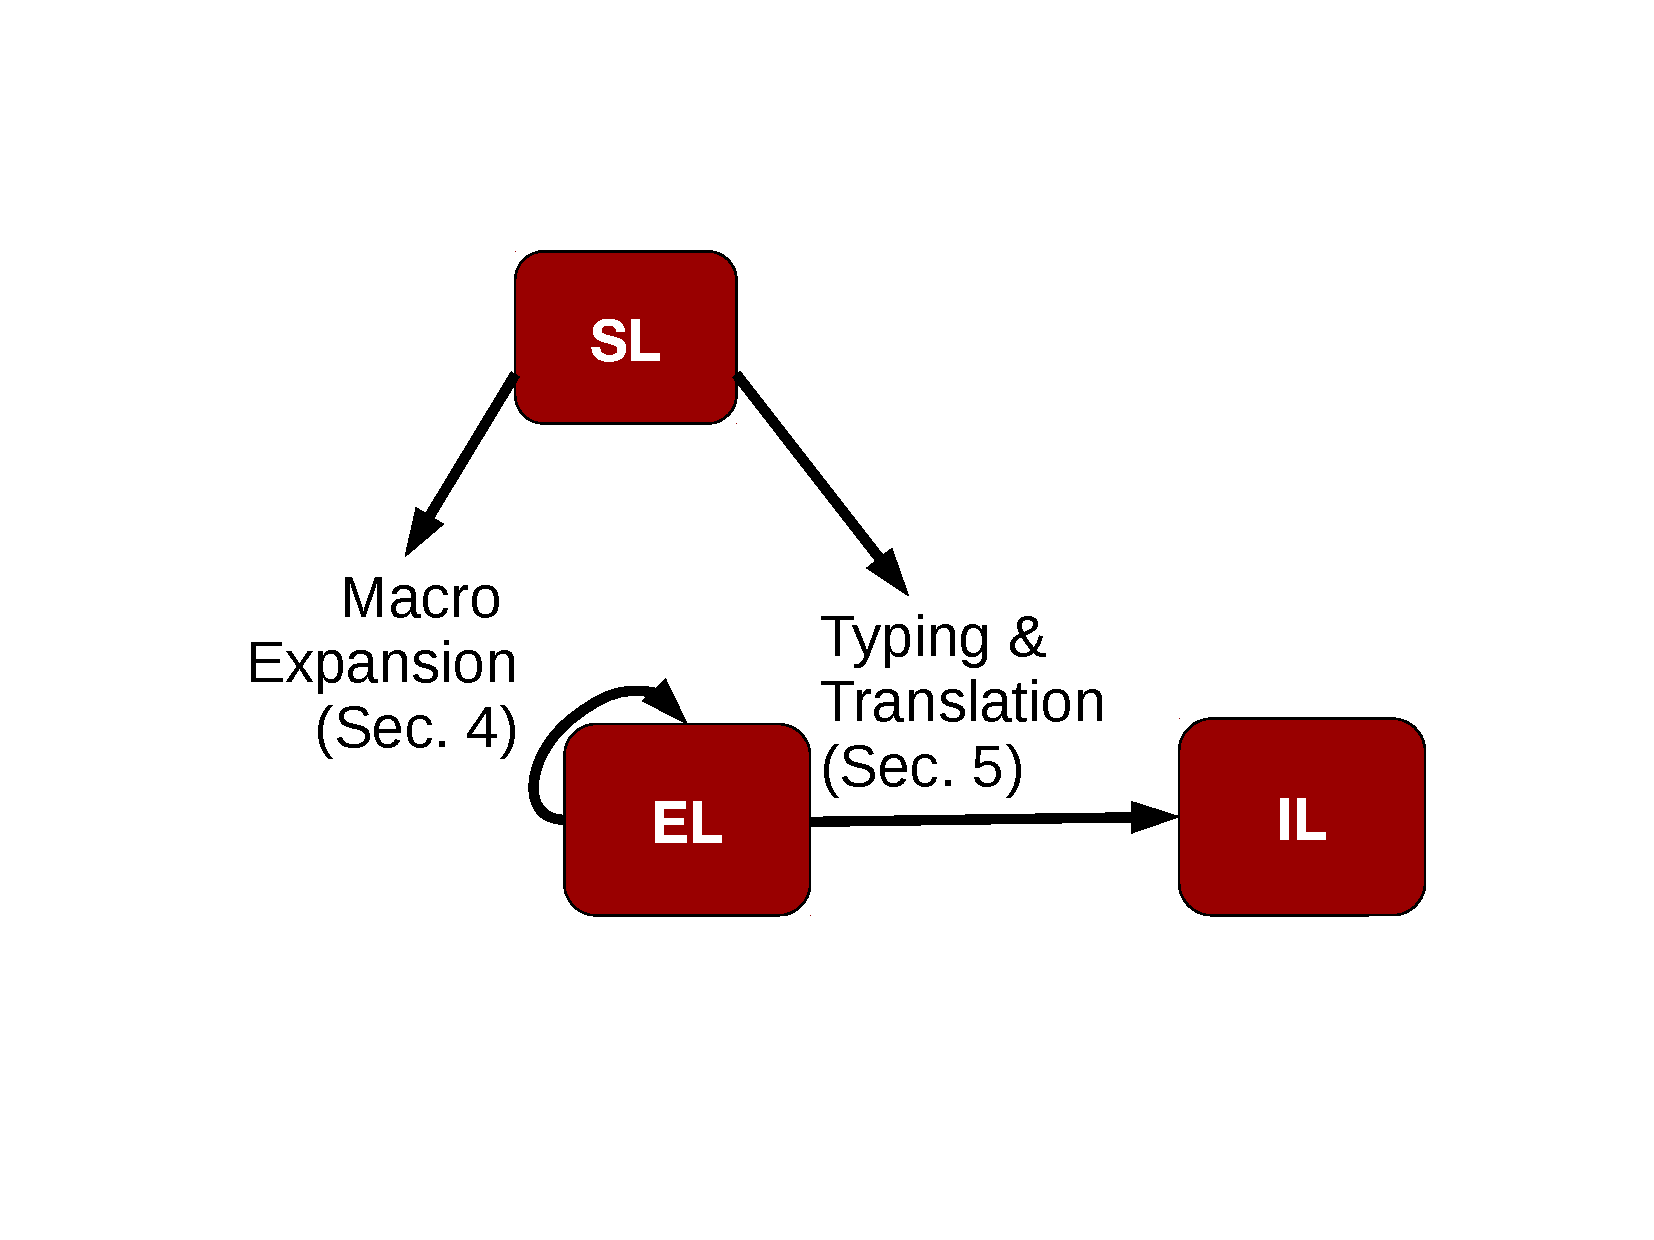
\includegraphics[scale=0.5,clip=true,trim=0 120 0 120]{overview.pdf}\vspace{-10px}
% \caption{A diagrammatic overview of the core language.}
% \vspace{5px}
% \label{fig:overview}
% \end{figure}

% \subsubsection{Internal Language}
% Programs ultimately evaluate as \emph{internal expressions}, $\iota$. Internal expressions are classified by \emph{internal types}, $\tau$, so the internal language forms a standard typed lambda calculus. For our purposes, it suffices to use the strictly evaluated polymorphic lambda calculus with nullary and binary product and sum types and recursive types as our IL. We assume in this proposal that the reader is familiar with this language (we follow \emph{PFPL} \cite{pfpl} directly). The main judgements in the static semantics of the IL take the following familiar form (omitting contexts for simplicity throughout this section):
% \\[1ex]
% $
% \begin{array}{ll}
% \textbf{Judgement Form} & \textbf{Pronunciation}\\
% \vdash \tau~\mathtt{itype} & \text{Internal type $\tau$ is valid.}\\
% \vdash \iota : \tau & \text{Internal expression $\iota$ is assigned internal type $\tau$.}
% \end{array}
% $\\

% \noindent
% The dynamic semantics are specified also in the standard manner as a transition system with  judgements of the following form:
% \\[1ex]
% $
% \begin{array}{ll}
% \textbf{Judgement Form} & \textbf{Pronunciation}\\
% \iota \mapsto \iota' & \text{Internal expression $\iota$ transitions to $\iota'$.}\\
% \iota~\mathtt{val} & \text{Internal expression $\iota$ is a value.}
% \end{array}
% $
% \\[1ex]
% The iterated transition judgement $\iota \mapsto^{*} \iota'$ is the reflexive, transitive closure of the transition judgement, and the evaluation judgement $\iota \Downarrow \iota'$ is derivable iff $\iota \mapsto^{*} \iota'$ and $\iota'~\mathtt{val}$. 

% Note that features like state, exceptions, basic concurrency primitives, scalars, arrays, I/O primitives and others characteristic of a first-stage compiler intermediate language would also be included in the IL in practice, and for several of these, this would affect the shape of the internal semantics. However, our design is largely insensitive to such details -- the only strict requirements are that the IL be type safe and support parametric type abstraction. To give a simple account of our novel contributions, we will stick to this small, familiar IL for the purposes of this work. %Features like record types and labeled sum types, on the other hand, are not built in.



% \subsubsection{External Language}
% The external language (EL) supports a richer syntax and type structure atop the IL. Most programmers will interact exclusively with the EL, so throughout this work, the words ``expression'' and ``type'' used without qualification refer to external expressions and types, respectively. The central judgements in the specification of the EL take the following form  (again omitting various contexts, which we will introduce progressively): 
% \\[1ex]
% $\begin{array}{ll}
% \textbf{Judgement Form} & \textbf{Pronunciation}\\
% \vdash \sigma~\mathtt{type} \leadsto \tau & \text{Static expression $\sigma$ is a type with translation $\tau$.}\\
% \vdash e \Rightarrow \sigma \leadsto \iota & \text{Expression $e$ synthesizes type $\sigma$ and has translation $\iota$.}\\
% \vdash e \Leftarrow \sigma \leadsto \iota & \text{Expression $e$ analyzes against type $\sigma$ and has translation $\iota$.}
% \end{array}
% $\\[1ex]The main points to note here are that:
% \begin{itemize}
% \item External types are distinct from internal types (thus distinguishing this style of specification from the Harper-Stone elaboration semantics for Standard ML \cite{Harper00atype-theoretic}).
% \item The expression typing judgements are \emph{bidirectional}, i.e. we make a judgemental distinction between \emph{type synthesis} (the type is an ``output'') and \emph{type analysis} (the type is an ``input'') \cite{Pierce:2000:LTI:345099.345100}. This will  allow us to explicitly specify how Verse's \emph{local type inference} works, and in particular, how it interacts with the primitives that we aim to introduce. Like Scala, we do not seek to support non-local type inference. %, primarily because it is not technically compatible with the primitives we will introduce (but also because we believe that compilers for languages that support only local type inference generate clearer error messages). 
% \item  The dynamic behavior of an external expression is determined directly by its translation to the IL, i.e. there is no separate transition system governing the dynamics of external expressions. 

% Proving type safety amounts to proving that the translation of every external expression of type $\sigma$ is an internal expression of type $\tau$, where $\tau$ is the translation of $\sigma$ (and thus, by type safety of the IL, evaluation does not ``go wrong''). This corresponds notionally to the idea of \emph{type-preserving compilation} in type-directed compilers \cite{tarditi+:til-OLD}.
% \end{itemize}

% \subsubsection{Static Language}
% Finally, the static language plays an important role in the semantics of the novel primitives that are the topic of this proposal. The static language is simply another typed lambda calculus consisting of \emph{static expressions}, $\sigma$, classified by \emph{sorts}\footnote{We use the word ``sort'' to avoid confusion with the phrase ``static type''. Our use of the  word ``sort'' should be considered distinct from the various other uses of this word found in the literature on programming languages.}, $\uppi$, according to the following judgements (the ``static statics''):
% \\[1ex]
% $
% \begin{array}{ll}
% \textbf{Judgement Form} & \textbf{Pronunciation}\\
% \vdash \uppi~\mathtt{sort} & \text{Sort $\uppi$ is valid.}\\
% \vdash \sigma :: \uppi & \text{Static expression $\sigma$ has sort $\uppi$.}
% \end{array}
% $\\

% \noindent
% The ``static dynamics'' are specified as a transition system with judgements of the following basic form (though again omitting some necessary contexts):
% \\[1ex]
% $
% \begin{array}{ll}
% \textbf{Judgement Form} & \textbf{Pronunciation}\\
% \sigma \mapsto \sigma' & \text{Static expression $\sigma$ transitions to $\sigma'$.}\\
% \sigma~\mathtt{sval} & \text{Static expression $\sigma$ is a static value.}\\
% \sigma~\mathtt{styerr} & \text{Static expression $\sigma$ raises an external type error.}
% \end{array}
% $
% \\[1ex]
% The iterated static transition judgement $\sigma \mapsto^{*} \sigma'$ is the reflexive, transitive closure of the static transition judgement, and the static evaluation judgement $\sigma \Downarrow \sigma'$ is derivable iff $\sigma \mapsto^{*} \sigma'$ and $\sigma'~\mathtt{sval}$. 

% As suggested by the form of the external type translation judgement above, external types are static expressions. More specifically, external types are static values of a primitive sort $\mathsf{Ty}$. We will return to how this works in Sec. \ref{sec:metamodules}. 
% %One might notice the similarities between the specifications of the SL and the IL. In fact, the SL is a conservative extension of our IL. In practice, one would not implement them separately, but formally, it is more convenient to specify them separately. 


% % The reason why we refer to the syntactic sort $\sigma$ as a ``static expression'' will become more clear later.

% %The main novelty of our work is that the Verse EL builds in very little syntax or type structure \emph{a priori}. %Instead, \textbf{metamodules} and \textbf{typed syntax macros} (TSMs) are expressive enough to render this unnecessary. Although metamodules are in some sense prior to TSMs, we will describe TSMs first, temporarily assuming that the EL does build in standard type structure, for pedagogical purposes. 
% \subsection{Module Language}

% The Verse module system is taken directly (up to small syntactic changes) from Standard ML, with which we assume a working familiarity for the purposes of this proposal \cite{harper1997programming,MacQueen:1984:MSM:800055.802036} (a related module system, e.g. OCaml's, would work just as well for our purposes). We will give examples of its use in Sec. \ref{sec:syntax} and Sec. \ref{sec:metamodules}.

% Formally, our approach will be to first specify our contributions assuming a language without an ML-style module system, then make modifications to this specification to make it compatible with the presence of a module system. Because it has been thoroughly studied in the literature, we will defer to prior work both here and in the dissertation for many formal details. In particular, it will suffice to assume that modules are being tracked by a suitable \emph{module context}, without detailing how this context is populated. %This context will be analagous to the \emph{named type context} specified in the papers just cited.% Instead, we will consider it abstractly where it interacts with the core language.%\todo{reminder that we are not going to re-specify the module system}



\section{Background}\label{sec:background}
%To begin, let us assume a standard, ML-like semantics for both the EL and SL and consider the EL's concrete syntax. 
Verse, like most contemporary languages, specifies a textual concrete syntax.\footnote{Although Wyvern specified a layout-sensitive concrete syntax, to avoid unnecessary distractions, we will describe a more conventional layout-insensitive concrete syntax for Verse.} %We have chosen to specify a layout-sensitive textual concrete syntax (i.e. newlines and indentation are not ignored). This design choice is not  fundamental to our proposed contributions, but it will be useful for cleanly expressing a class of examples that we plan to discuss later. We plan to specify some novel aspects of Verse's concrete syntax with an \emph{Adams grammar} \cite{Adams:2013:PPI:2429069.2429129} (such a specification for Wyvern, which has a very similar syntax, can be found in \cite{TSLs}), but for the purposes of this proposal, we will simply introduce Verse's concrete syntax by example as we go on. %For constructs that have an obvious analog in ML, we will omit a detailed explanation.
Because the purpose of this syntax is to serve as the programmer-facing user interface of the language, it is common practice to build in  derived syntactic forms (colloquially, \emph{syntactic sugar}) that capture common idioms more concisely or ``naturally''. % (i.e. considering cognitive dimensions \cite{green1996usability}). 
For example, derived list syntax is built in to many functional languages, so that instead of having to write out \lstinline{Cons(1, Cons(2, Cons(3, Nil)))}, the programmer can equivalently write \lstinline{[1, 2, 3]}. Many languages go beyond this, building in derived syntax associated with various other types of data, like vectors (the SML/NJ dialect of SML), arrays (OCaml), monadic commands (Haskell), syntax trees (Scala, F\#), XML documents (Scala, Ur/Web) and SQL queries (F\#, Ur/Web). %This is a rather \emph{ad hoc} process.% discussed previously, the usual approach is to require that the language designer build in new derived syntactic forms. %The desugaring from the latter to the former is specified by the language itself. %Typically, the language designer controls what forms of derived syntax are built in to the language.

Verse takes a less \emph{ad hoc} approach -- rather than privileging  particular library constructs with primitive syntactic support, Verse exposes primitives that allow library providers to introduce new expansion logic on their own, in a safe and modular manner. %Lists need no special consideration from the language specification.
%The purpose of this section is to  a and then introduce Verse's syntax extension mechanisms. %For forms with a clear analogy to a form in Standard ML, we will assume the  semantics are analagous without providing details.

We will begin in Sec. \ref{sec:examples} by detailing another example for which such a mechanism would be useful: regular expression (regex) patterns expressed using abstract data types. We will refer to this example throughout the proposal. In Sec. \ref{sec:syntax-existing}, we discuss how the usual approach of using dynamic string parsing to introduce regex patterns is not ideal. We also survey existing alternatives to dynamic string parsing, finding that they involve an unacceptable loss of modularity and other undesirable trade-offs. In Secs. \ref{sec:tsms} and \ref{sec:tsls}, we introduce our proposed alternatives -- \emph{typed syntax macros} (TSMs) and the related \emph{type-specific languages} (TSLs) -- and discuss how they resolve these issues (as well as some limitations that they have). We  also give an overview of how TSMs are formally specified. We give a concrete timeline for the remaining work in Sec. \ref{sec:syntax-timeline}, and conclude in Sec. \ref{sec:conclusion}.


\subsection{Motivating Example: Regular Expression Syntax}\label{sec:examples}\label{sec:syntax-examples}
Let us begin by taking the perspective of a regular expression library provider. We assume the reader has some familiarity with regular expressions \cite{Thompson:1968:PTR:363347.363387} and Standard ML \cite{harper1997programming}. We will discuss a standard variant of regular expressions that supports marking \emph{captured groups} (with parentheses in the concrete syntax) to make certain examples more interesting.

\paragraph{Abstract Syntax} The abstract syntax of {patterns}, $r$, over strings, $s$, is specified below:\[r ::= \textbf{empty} ~|~ \textbf{str}(s) ~|~ \textbf{seq}(r; r) ~|~ \textbf{or}(r; r) ~|~ \textbf{star}(r) ~|~ \textbf{group}(r)\]
One way to express this abstract syntax is by defining a recursive sum type \cite{pfpl}. Verse supports these as datatypes:

\begin{lstlisting}[numbers=none]
datatype Rx {
    Empty | Str of string | Seq of Rx * Rx 
    | Or of Rx * Rx | Star of Rx | Group of Rx
}
\end{lstlisting}

However, there are some reasons not to expose this representation of patterns directly to clients. First, regular expression patterns are usually identified up to their reduction to a normal form. For example, $\textbf{seq}(\textbf{empty}, r)$ has normal form $r$. It might be useful for patterns with the same normal form to be  indistinguishable from the perspective of client code. Second, it can be useful for performance reasons to maintain additional data alongside regexes (e.g. a corresponding finite automata) without exposing this ``implementation detail'' to clients. Indeed, there may be many ways to represent regular expression patterns, each with different performance trade-offs. For these reasons, a better approach in Verse, as in ML, is to abstract over the choice of representation using  the module system's support for type abstraction. In particular, we can define the following \emph{module signature}, where the type of patterns, \lstinline{t}, is held abstract:
%Notice that it exposes an interface otherwise  to the one available using a case type:

\begin{lstlisting}[deletekeywords={case},numbers=none]
signature RX = sig {
  type t
  val Empty : t
  val Str : string -> t
  val Seq : t * t -> t
  val Or : t * t -> t
  val Star : t -> t
  val Group : t -> t
  val case : (
    t -> {
    	Empty : 'a,
    	Str : string -> 'a,
    	Seq : t * t -> 'a,
    	Or : t * t -> 'a,
    	Star : t -> 'a,
    	Group : t -> 'a
    } -> 'a
}
\end{lstlisting}
 Clients of any module \lstinline{R} that has been sealed against \lstinline{RX}, written \lstinline{R :> RX}, manipulate patterns as values of the type \verb|R.t| using the interface described by this signature. The identity of the type \lstinline{R.t} is held abstract outside the module during typechecking (i.e. it acts as a newly generated type). As a result, the burden of proving that there is no way to use the case analysis function to distinguish patterns with the same normal form is local to the module, and implementation details do not escape (and can thus evolve freely). %The details are standard and not particularly relevant for our purposes, so we omit them here.

\paragraph{Concrete Syntax} The abstract syntax of patterns is too verbose to be practical  in all but the most trivial examples, so programmers conventionally write patterns using a more concise concrete syntax. For example, the concrete syntax \lstinline{A|T|G|C} corresponds to the following much more verbose pattern expression (assuming some module \lstinline{R : RX} is in scope here and in the remainder of the document):
\begin{lstlisting}[numbers=none,mathescape=|]
R.Or(R.Str "SSTRAESTR", R.Or(R.Str "SSTRTESTR", R.Or(R.Str "SSTRGESTR", R.Str "SSTRCESTR")))
\end{lstlisting} 



% \begin{figure}
% \begin{center}
% 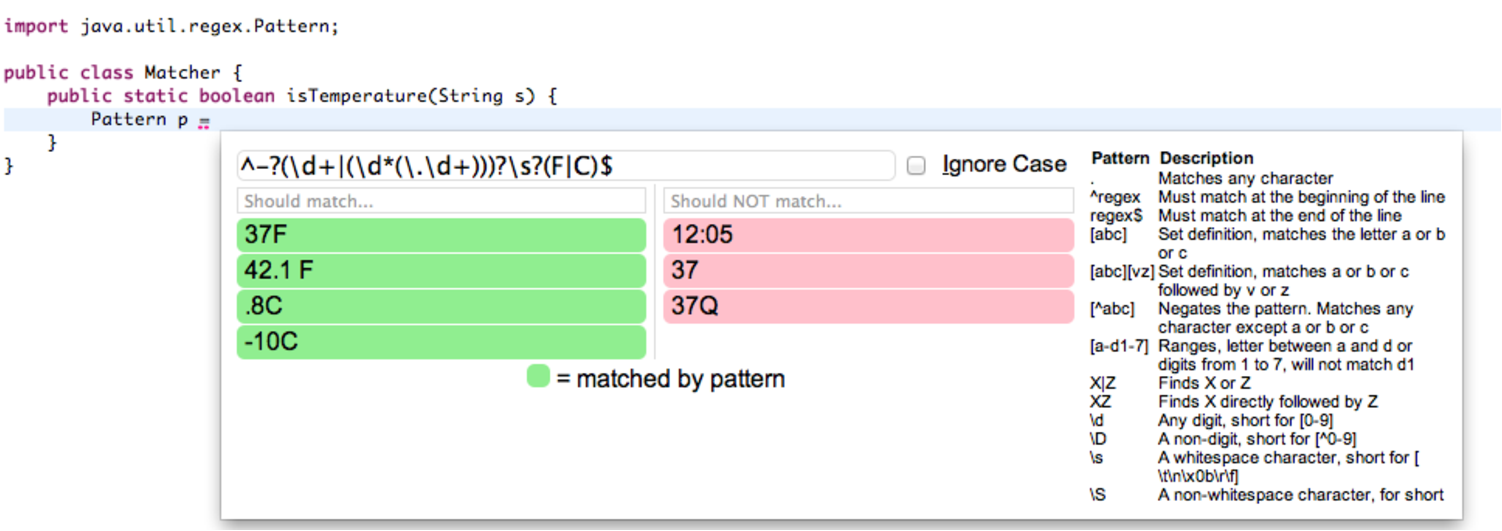
\includegraphics[scale=.55]{regex-palette.pdf}\\
% $\Downarrow$ \text{(pressing \textbf{Enter})}\\
% 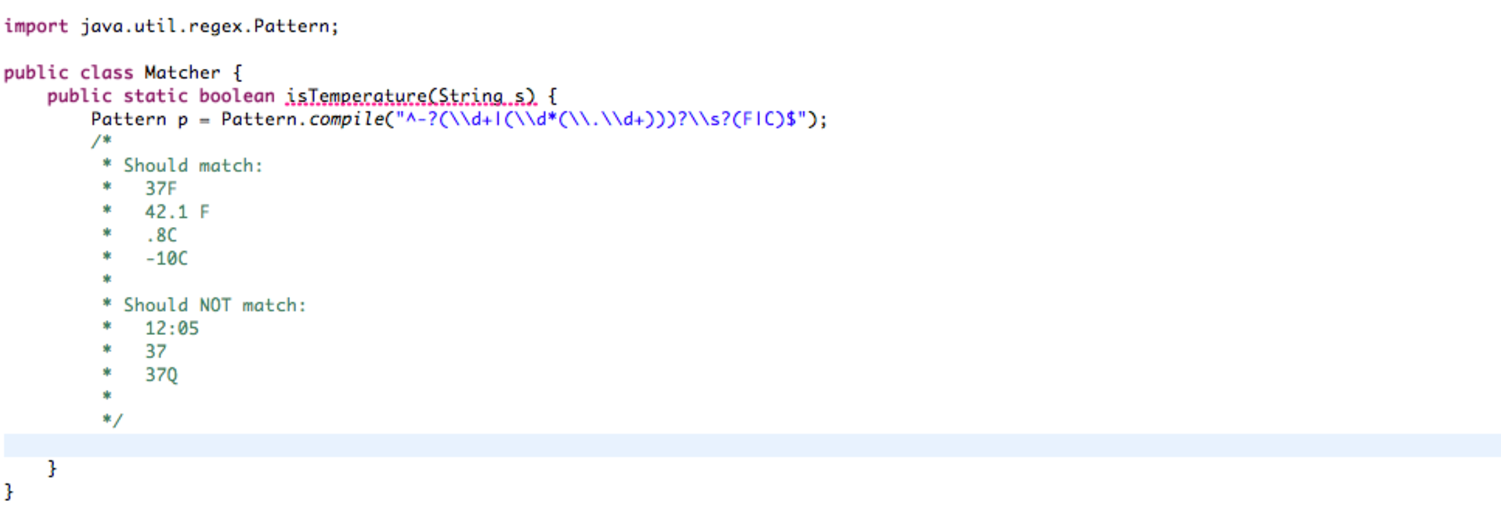
\includegraphics[scale=.55]{regex-code-generated.pdf}
% \end{center}
% \vspace{-20px}
% \caption{An example of type-specific editor services, here shown for Java.}
% \label{fig:regex-palette}
% %\vspace{-10px}
% \end{figure}

%In a conventional \emph{monolithic} programming system, support for each of these features would need to be built into the language and tools. 

\subsection{Existing Approaches}\label{sec:syntax-existing}\label{sec:syntax-existing-approaches}
\subsubsection{Dynamic String Parsing}
To expose this more concise concrete syntax for regular expression patterns to clients, the most common approach is to provide a function that parses strings to produce patterns. Because, as just mentioned, there  may be many implementations of the \lstinline{RX} signature, the usual approach is to define a parameterized module (a.k.a. a \emph{functor} in SML) defining utility functions like this abstractly:

\begin{lstlisting}[numbers=none]
module RXUtil(R : RX) => mod {
  fun parse(s : string) : R.t => (* ... regex parser here ... *)
}
\end{lstlisting}
This allows a client of any module \lstinline{R : RX} to use the following definitions:
\begin{lstlisting}[numbers=none]
let module RUtil = RXUtil(R)
let val rxparse = RUtil.parse
\end{lstlisting}
to construct patterns like this:
\begin{lstlisting}[numbers=none]
rxparse "SSTRA|T|G|CESTR"
\end{lstlisting}
 %Again, none of our goals are comprehensively achieved.
Unfortunately, this approach is imperfect for several reasons:
\begin{enumerate} 
\item First, there are syntactic conflicts between string escape sequences and pattern escape sequences. For example, the following is not a well-formed term:
\begin{lstlisting}[numbers=none,mathescape=|]
let val ssn = rxparse "SSTR\d\d\d-\d\d-\d\d\d\dESTR"
\end{lstlisting}
When compiling an expression like this, the client would see an error message like \verb|error: illegal escape character|\footnote{This is the error message that \texttt{javac} produces. When compiling an analagous expression using SML of New Jersey (SML/NJ), we encounter a more confusing error message: \texttt{Error: unclosed string}.}, because \verb|\d| is not a valid string escape sequence. In a small lab study, we observed that this class of error often confused even experienced programmers if they had not used regular expressions recently \cite{Omar:2012:ACC:2337223.2337324}. One workaround has higher syntactic cost -- we must double all backslashes:
\begin{lstlisting}[numbers=none]
let val ssn = rxparse "SSTR\\d\\d\\d-\\d\\d-\\d\\d\\d\\dESTR"
\end{lstlisting}

Some languages, anticipating such modes of use, build in alternative string forms that leave escape sequences uninterpreted. For example, OCaml supports the following, which has only a constant syntactic cost:
\begin{lstlisting}[numbers=none]
let val ssn = rxparse {rx|SSTR\d\d\d-\d\d-\d\d\d\dESTR|rx}
\end{lstlisting}

\item The next problem is that dynamic string parsing mainly decreases the syntactic cost of complete patterns. Patterns constructed compositionally cannot easily benefit from this technique. For example, consider the following function from strings to patterns:
\begin{lstlisting}[numbers=none]
fun example(name : string) => 
  R.Seq(R.Str(name), R.Seq(rxparse "SSTR: ESTR", ssn)) (* ssn as above *)
\end{lstlisting}
%We needed to use both dynamic string parsing and explicit applications of pattern constructors to achieve the intended semantics. 
Had we built derived syntax for regular expression patterns into the language primitively (following Unix conventions of using forward slashes as delimiters), we could have used \emph{splicing syntax}:
\begin{lstlisting}[numbers=none]
fun example_shorter(name : string) => /SURL@EURLnameSURL: %EURLssn/
\end{lstlisting}
An identifier (or parenthesized expression, not shown) prefixed with an \lstinline{@} is a spliced string, and one prefixed with a \lstinline{%} is a spliced pattern.

It is difficult to capture idioms like this using dynamic string parsing, because strings cannot contain sub-expressions directly. 

%(we will see an example of syntax that does capture such idioms below).

\item For functions like \lstinline{example} where we are constructing patterns on the basis of data of type \lstinline{string}, using strings coincidentally to introduce patterns tempts programmers to use string concatenation in subtly incorrect ways. For example, consider the following seemingly more readable definition of \lstinline{example}:
\begin{lstlisting}[numbers=none,escapechar=~]
fun example_bad(name : string) => 
  rxparse (name ^ {rx|SSTR: \d\d\d-\d\d-\d\d\d\dESTR|rx})
\end{lstlisting}
%The (unstated) intent here was to treat \lstinline{name} as a sub-pattern matching only itself, but this is not the observed behavior when \lstinline{name} contains special characters that have other meanings in patterns.

Both \lstinline{example} and \lstinline{example_bad} have the same type and behave identically at many inputs, particularly ``typical'' inputs (i.e. alphabetic names). It is only when the input \lstinline{name} contains special characters that have meaning in the concrete syntax of patterns that a problem arises. 

In applications that query sensitive data, mistakes like this lead to \emph{injection attacks}, which are among the most common and catastrophic security threats on the web today \cite{owasp2013}. These are, of course, a consequence of the programmer making a mistake in an effort to decrease syntactic cost, but proving that mistakes like this have not been made involves reasoning about complex run-time data flows, so it is once again notoriously difficult to automate. If our language supported derived syntax for patterns, this kind of mistake would be substantially less common (because \lstinline{example_shorter} has lower syntactic cost than \lstinline{example_bad}).
 %Ultimately, of course, mistakes like this are the fault of a programmer using a flawed heuristic, and they could be avoided with discipline. The problem is once again that it is difficult to detect violations of this discipline automatically. 

 %Ideally, our library would be able to make it more difficult to inadvertently introduce subtle security bugs like this.
\item The next problem is that pattern parsing does not occur until the pattern is evaluated. For example, the following malformed pattern will only trigger an exception when this expression is evaluated during the full moon: %Achieving this goal is an explicit goal of this proposal, so we are obviously not happy with this.

\begin{lstlisting}[numbers=none]
case(moon_phase) {
    Full => rxparse "SSTR(GCESTR" (* malformedness not statically detected *)
  | _ => (* ... *)
}
\end{lstlisting}
Though malformed patterns can sometimes be discovered dynamically via testing, empirical data gathered from large open source projects suggests that there remain many malformed regular expression patterns that are not detected by a project's test suite ``in the wild'' \cite{spishak2012type}. 

Statically verifying that pattern formation errors will not dynamically arise requires reasoning about arbitrary dynamic behavior. This is an undecidable verification problem in general and can be difficult to even partially automate. In this example, the verification procedure would first need to be able to establish that the variable \lstinline{rxparse} is equal to the parse function \lstinline{RUtil.parse}. If the string argument had not been written literally but rather computed, e.g. as \lstinline{"SSTR(GESTR" ^ "SSTRCESTR"} where \lstinline{^} is the string concatenation function applied in infix style, it would also need to be able to establish that this expression is equivalent to the string \lstinline{"SSTR(GCESTR"}. For patterns that are dynamically constructed based on input to a function, evaluating the expression statically (or, more generally, in some earlier ``stage'' of evaluation \cite{Jones:Gomard:Sestoft:93:PartialEvaluation}) also does not suffice. 

Of course, asking the client to provide a proof of well-formedness would defeat the purpose of lowering syntactic cost.

In contrast, were our language to primitively support  derived pattern syntax, pattern parsing would occur at compile-time and so malformed patterns would produce a compile-time error.

\item Dynamic string parsing also necessarily incurs dynamic cost. Regular expression patterns are common when processing large datasets, so it is easy to inadvertently incur this cost repeatedly. For example, consider mapping over a list of strings:
\begin{lstlisting}[numbers=none]
map exmpl_list (fn s => rxmatch (rxparse "SSTRA|T|G|CESTR") s)
\end{lstlisting}
To avoid incurring the parsing cost for each element of \lstinline{exmpl_list}, the programmer or compiler must move the parsing step out of the closure (for example, by eta-reduction in this simple example).\footnote{Anecdotally, in major contemporary compilers, this optimization is not automatic.} If the programmer must do this, it can (in more complex examples) increase syntactic cost and cognitive cost by moving the pattern itself far away from its use site. Alternatively, an appropriately tuned memoization (i.e. caching) strategy could be used to amortize some of this cost, but it is difficult to reason compositionally about performance using such a strategy. %If the programmer does it, it can sometimes make the program more difficult to read. 

%This too is difficult if a portion of the pattern is dynamically generated. % Regular expressions are often used across large datasets in scientific applications, so the absolute peformance penalty can be non-trivial.

In contrast, were our language to primitively support derived pattern syntax, the expansion would be computed at compile-time and incur no dynamic cost.
\end{enumerate}

% \begin{enumerate}
% \item \textbf{Conventional Concrete Syntax.} Patterns must be written in exactly the conventional manner, shown in blue below. Curly braces serve as an ``unquote'' form to splice one pattern into another:
% \begin{lstlisting}[numbers=none]
% let N : Pattern = /SURLA|T|G|CEURL/
% let BisI : Pattern = /SURLGC{EURLNSURL}GCEURL/
% let twoDigits : Pattern = /SURL\d\dEURL/\end{lstlisting}

% %The choice of delimiter, i.e. matching forward slashes here, is not important.
% %The cognitive load of reading and writing patterns is low and patterns are parsed once at compile-time. 
% \item \textbf{Compile-Time Parsing.} Pattern parsing must occur at compile-time, i.e. it must not incur run-time cost and malformed patterns, e.g. \lstinline{/SURLGC(EURL/}, must result in {compile-time} errors no matter where they appear in the program. 
% \item \textbf{Security By Default.} Strings must not be treated as patterns, nor used idiomatically to construct patterns. For example, the function below must be ill-typed because \lstinline{name} is not of type \lstinline{Pattern}:
% \begin{lstlisting}[numbers=none]
% fun example(name : string) : Pattern
%   let twoDigits : Pattern = /SURL\d\dEURL/
%   /SURL{EURLnameSURL}: {EURLtwoDigitsSURL}EURL/
% \end{lstlisting}
%     It is also acceptable for \lstinline{example("SSTR[a-z]ESTR")} to be equivalent to \lstinline{/SURL\[a-z\]: \d\d/}, i.e. strings are treated as patterns matching only themselves. 
% It is \emph{not} acceptable for \lstinline{example("SSTR[a-z]ESTR")} to be equivalent to \lstinline{/SURL[a-z]: \d\d/}. 

%     This is a security issue because if \lstinline{name} is derived from user input, such confusion could lead to \emph{injection attacks}, which are both common and catastrophic when using regular expression libraries that fail to achieve these goals, discussed below \cite{owasp2013}. 
%   %\item A more advanced semantics might ensure that out-of-bounds backreferences to a captured group do not occur \cite{spishak2012type}. For example, we would want \verb|BisI|, above, to have the more precise type \lstinline{Pattern(1)}, i.e. a pattern with one captured group. 
% % \end{enumerate}
% %When an error is found, an intelligible error message is provided.
% %\item An \textbf{implementation} that partially or fully compiles known regular expressions into the efficient internal representation that will be used by the regular expression matching engine (e.g., a finite automata \cite{Thompson:1968:PTR:363347.363387}) ahead of time. In most languages, this compilation step occurs at run-time, even if the pattern is fully known at compile-time, thereby introducing performance overhead into programs. If the developer is not careful to cache compiled representations, regular expressions used repeatedly in a program might be needlessly re-compiled on each use. %By performing this step ahead-of-time, these dangers can be avoided.
% %\item A range of \textbf{editor services} that support syntax highlighting for patterns, retrieval of relevant documentation, interactive testing, and pattern extraction from example strings have been shown to be helpful for programmers when working with complex regular expressions \cite{ACC_VLHCC}. An example of some of these is shown in Figure \ref{fig:regex-palette}: the editor service shown helps programmers generate correct code, here via the Java standard library's implementation of regular expressions (discussed below).
% \end{enumerate}
% Let us consider the ways that providers of regular expression libraries commonly choose to define the type \verb|Pattern|: as synonymous to \lstinline{string}, as a recursive sum type, or as an abstract type.

% \vspace{-5px}
% \paragraph{Patterns as Strings} The most na\"ive choice is to define \lstinline{Pattern} as synonymous to \lstinline{string}:

% \begin{lstlisting}[numbers=none]
% type Pattern = string
% \end{lstlisting}
% The only reason to consider this definition is that it allows us to approximate pattern syntax using standard string literal syntax:

% \begin{lstlisting}[numbers=none]
% let N : Pattern = "SSTRA|T|G|CESTR"
% \end{lstlisting}
% To splice one pattern into another, we can perform string concatenation:
% \begin{lstlisting}[numbers=none,escapechar=|]
% let BisI : Pattern = "SSTRGCESTR" ^ N ^ "SSTRGCESTR"
% \end{lstlisting}
% or use string interpolation (as in Scala or SML/NJ using quotation/antiquotation \cite{SML/Quote}):
% \begin{lstlisting}[numbers=none,mathescape=|]
% let BisI : Pattern = s"SSTRGC${ESTRNSSTR}GCESTR"
% \end{lstlisting}

% Though this comes close, goal 1 is not truly achieved because the syntax of strings can conflict with the syntax for patterns. 

% Goal 2 is not achieved because parsing occurs only at run-time when we match a string against a pattern (worse, every time we do so unless the implementation uses an effective caching strategy).

% Goal 3 is also not achieved because the following code typechecks:
% \begin{lstlisting}[numbers=none,mathescape=|]
% fun example_bad_1(name : string) : Pattern
%   let twoDigits : Pattern = "SSTR\\d\\dESTR"
%   s"SSTR${ESTRnameSSTR}-${ESTRtwoDigitsSSTR}"ESTR
% \end{lstlisting}
% but \lstinline{example_bad_1("SSTR[a-z]ESTR")} evaluates to \lstinline{"SSTR[a-z]-\\d\\dESTR"}.



% \paragraph{Patterns as Recursive Sums} A more semantically justifiable strategy is to define \lstinline{Pattern} as a recursive sum type  \cite{pfpl}. Verse supports these in the form of case types, which are analagous to datatypes in ML:

% \begin{lstlisting}[numbers=none]
% casetype Pattern
%   Empty
%   Str of string
%   Seq of Pattern * Pattern
%   Or of Pattern * Pattern
%   Star of Pattern  
% \end{lstlisting}

% More generally, we can hold the representation of patterns abstract while exposing an isomorphic interface to clients by defining an abstract type in a {module} opaquely ascribed the following {module type} (a.k.a. \emph{signature} in SML): % exposes the constructors and case analysis as functions:

% \begin{lstlisting}[deletekeywords={case},numbers=none]
% module type PATTERN
%   type t
%   val Empty : t
%   val Str : string -> t
%   val Seq : t * t -> t
%   val Or : t * t -> t
%   val Star : t -> t
%   val case : (
%     'a -> 
%     (string -> 'a) ->
%     (t * t -> 'a) ->
%     (t * t -> 'a) ->
%     (t -> 'a) ->
%     'a)
% \end{lstlisting}
% The client of any module \lstinline{P : PATTERN} can define \verb|Pattern| as synonymous to \verb|P.t|: 
% \begin{lstlisting}[numbers=none]
% type Pattern = P.t
% \end{lstlisting}



%The first one might not be found incorrect without rigorous testing with unexpected inputs. Goal 3 expresses the ideal of designing a language where security does not require considering such subtle issues extralinguistically.%This is precisely why injection attacks are so difficult to detect.

% The dialect of Standard ML implemented by SML/NJ, recognizing that directly using constructors is often less than ideal, provides a facility for quotation/antiquotation \cite{SML/Quote}, which if introduced into Verse could be used as follows:
% \begin{lstlisting}[numbers=none,escapechar=|,mathescape=|]
% fun example(p : string)
%   let twoDigits = P.qparse `SQT\d\dEQT`
%   P.qparse `SQT^(EQTP.Str(p)SQT)-^(EQTtwoDigitsSQT)EQT`
% \end{lstlisting}

% Here, backticks are used to indicate a quoted term within which carets serve as an antiquote operator. This still represents a  compromise against goal 1. The most serious problem is that, once again, parsing does not occur until run-time. There are also  conflicts between quotation syntax and pattern syntax, i.e. \verb|^| conventionally means character set negation inside patterns, which conflicts with antiquotation here. This mechanism also does not support antiquotation at more than one type, so we could not define the antiquote operator to insert the \verb|Str| constructor automatically, as suggested in goal 3. %For syntax that necessary involves antiquotation at multiple types (e.g. concrete syntax for a programming language with multiple syntactic sorts, HTML which might include Javascript and CSS, and others), this 

The problems above are not unique to regular expression patterns. Whenever a library encourages the use of dynamic string parsing to address the issue of syntactic cost (which is, fundamentally, not a dynamic issue), these problems arise. %Strings are, simply put, not ideally suited for this task. 
	This fact has motivated much research on reducing the need for dynamic string parsing \cite{Bravenboer:2007:PIA:1289971.1289975}. Existing alternatives can be broadly classified as being based on either \emph{direct syntax extension} or \emph{static term rewriting}. We describe these next, in Secs. \ref{sec:syntax-extension} and \ref{sec:term-rewriting} respectively.% We summarize the most relevant work below.

\subsubsection{Direct Syntax Extension}\label{sec:syntax-extension}
One tempting alternative to dynamic string parsing is to use a system that gives the users of a language the power to directly extend its concrete syntax with new derived forms. %for regular expression patterns.% for patterns.

The simplest such systems are those where the elaboration of each new syntactic form is defined by a single rewrite rule. For example, Gallina, the ``external language'' of the Coq proof assistant, supports such extensions \cite{Coq:manual}. A formal account of such a system has been developed by Griffin \cite{5134}. Unfortunately, a single equation is not enough to allow us to express pattern syntax following the usual conventions. For example, a system like Coq's cannot handle escape characters, because there is no way to programmatically examine a form when generating its expansion.

Other syntax extension systems are more flexible. For example, many are based on context-free grammars, e.g.  Sugar* \cite{erdweg2013framework} and Camlp4 \cite{ocaml-manual} (amongst many others). Other systems give library providers direct programmatic access to the parse stream, like Common Lisp's \emph{reader macros} \cite{steele1990common} (which are distinct from its term-rewriting macros, described in Sec. \ref{sec:term-rewriting} below) and Racket's preprocessor \cite{Flatt:2012:CLR:2063176.2063195}. All of these would allow us to add pattern syntax into our language's grammar, perhaps following Unix conventions and supporting splicing syntax as described above:
\begin{lstlisting}[numbers=none]
let val ssn = /SURL\d\d\d-\d\d-\d\d\d\dEURL/
fun example_shorter(name : string) => /SURL@EURLnameSURL: %EURLssn/
\end{lstlisting}
%The body of this function elaborates to the body of \lstinline{example_fixed} as shown above. 
%Had we mistakenly written \lstinline{%name}, we would encounter only a static type error, rather than the  silent injection  vulnerability discussed above. 

We sidestep the problems of dynamic string parsing described above  when we directly extend the syntax of our language using any of these systems. Unfortunately, direct syntax extension introduces serious new problems. First, the systems mentioned thus far cannot guarantee that {syntactic conflicts} between such extensions will not arise. As stated directly in the  Coq manual: ``mixing different symbolic notations in [the] same text may cause serious parsing ambiguity''. If another library provider used similar syntax for a different implementation or variant of regular expressions, or for some other unrelated construct, then a client could not simultaneously use both libraries at the same time. So properly considered, every combination of extensions introduced using these mechanisms creates a \emph{de facto} syntactic dialect of our language. The benefit of these systems is only that they lower the implementation cost of constructing syntactic dialects. % Resolving such parsing amibiguities is left to each client of the library. 

In response to this problem, Schwerdfeger and Van Wyk developed a modular analysis that accepts only context-free grammar extensions that begin with an identifying starting token and obey certain constraints on  the follow sets of base language's non-terminals \cite{conf/pldi/SchwerdfegerW09}. Extensions that specify distinct starting tokens and that satisfy these constraints can be used together in any combination without the possibility of syntactic conflict. However, the most natural starting tokens like \lstinline{rx} cannot be guaranteed to be unique. To address this problem, programmers must agree on a convention for defining ``globally unique identifiers'', e.g. the common URI convention used on the web and by the Java packaging system. However, this forces us to use a more verbose token like \lstinline{edu_cmu_verse_rx}. There is no simple way for clients of our extension to define scoped abbreviations for starting tokens because this mechanism operates purely at the level of the context-free grammar.

Putting this aside, we must also consider another modularity-related question: which particular module should the expansion use? Clearly, simply assuming that some module identified as \lstinline{R} matching \lstinline{RX} is in scope is a brittle solution. In fact, we should expect that the system actively prevents such capture of specific variable names to ensure that variables (here, module variables) can be freely renamed. Such a \emph{hygiene discipline} is well-understood only when performing term-to-term rewriting (discussed below) or in simple language-integrated rewrite systems like those found in Coq. For mechanisms that operate strictly at the level of context-free grammars or the parse stream, it is not clear how one could address this issue. The onus is then on the library provider to make no assumptions about variable names and instead require that the client explicitly identify the module they intend to use as an ``argument'' within the newly introduced form:
\begin{lstlisting}[numbers=none]
let val ssn = edu_cmu_verse_rx R /SURL\d\d\d-\d\d-\d\d\d\dEURL/
\end{lstlisting}

Another problem with the approach of direct syntax extension is that, given an unfamiliar piece of syntax, there is no straightforward method for determining what type it will have, causing difficulties for both humans (related to code comprehension) and tools. 

\subsubsection{Static Term Rewriting}\label{sec:term-rewriting}
An alternative approach is to leave the concrete syntax of the language fixed, but repurpose it for novel ends using a \emph{local term-rewriting system}. The LISP macro system \cite{Hart63a} is perhaps the most prominent example of such a system. Early variants of this system suffered from the problem of unhygienic variable capture just described, but  later variants, notably in the Scheme dialect of LISP, brought support for enforcing hygiene \cite{Kohlbecker86a}. In languages with a richer static type discipline, variants of macros that restrict rewriting to a particular type and perform the rewriting statically have also been studied \cite{Herman10:Theory,ganz2001macros} and integrated into languages, e.g. MacroML \cite{ganz2001macros} and Scala \cite{ScalaMacros2013}. 

The most immediate problem with using these for our example is that we are not aware of any such statically-typed macro system that integrates cleanly with an ML-style module system. In other words, macros cannot be parameterized by modules. However, let us imagine such a macro system. We could use it to repurpose string syntax  as follows:
\begin{lstlisting}[numbers=none]
let val ssn = rx R {rx|SSTR\d\d\d-\d\d-\d\d\d\dESTR|rx}
\end{lstlisting}

The definition of the macro \lstinline{rx} might look like this:
\begin{lstlisting}
macro rx[Q : RX](e) at Q.t {
  static fun f(e : Exp) : Exp => case(e) {
      StrLit(s) => (* regex parser here *)
    | BinOp(Caret, e1, e2) => `SQTQ.Seq(Q.Str(%EQTe1SQT), %(EQTf e2SQT))EQT`
    | BinOp(Plus, e1, e2) => `SQTQ.Seq(%(EQTf e1SQT), %(EQTf e2SQT))EQT`
    | _ => raise Error
  }
}
\end{lstlisting}

Here, \lstinline{rx} is a macro parameterized by a module matching \lstinline{rx} (we identify it as \lstinline{Q} to emphasize that there is nothing special about the identifier \lstinline{R}) and taking a single argument, identified as \lstinline{e}. The macro specifies a type annotation, \lstinline{at Q.t}, which imposes the constraint that the expansion the macro statically generates must be of type \lstinline{Q.t} for the provided parameter \lstinline{Q}. This expansion is generated by a \emph{static function} that examines the syntax tree of the provided argument (syntax trees are of a type \lstinline{Exp} defined in the standard library; cf. SML/NJ's visible compiler \cite{SML/VisibleCompiler}). If it is a string literal, as in the example above, it statically parses the literal body to generate an expansion (the details of the parser, elided on line 3, would be entirely standard). 
By parsing the string statically, we avoid the problems of dynamic string parsing for statically-known patterns. 

For patterns that are constructed compositionally, we need to get more creative. For example, we might repurpose the infix operators that are normally used for other purposes to support string and pattern splicing, e.g. as follows:

\begin{lstlisting}[numbers=none,escapechar=|]
fun example_using_macro(name : string) => 
  rx R (name ^ "SSTR: ESTR" + ssn)
\end{lstlisting}

The binary operator \lstinline{^} is repurposed to indicate a spliced string and \lstinline{+} is repurposed to indicate a spliced pattern. The logic for handling these forms can be seen above on lines 4 and 5, respectively. We assume that there is derived syntax available at the type \lstinline{Exp}, i.e. \emph{quasiquotation} syntax as in Lisp \cite{Bawd99a} and Scala \cite{shabalin2013quasiquotes}, here delimited by backticks and using the prefix \lstinline{%} to indicate a spliced value (i.e. unquote). 

Having to creatively repurpose existing forms in this way limits the effect a library provider can have on syntactic cost (particularly when it would be desirable to express conventions that are quite different from the conventions adopted by the language). It also can create confusion for readers expecting parenthesized expressions to behave in a consistent manner. However,  this approach is preferable to direct syntax extension because it avoids many of the problems discussed above: there cannot be syntactic conflicts (because the syntax is not extended at all), we can define macro abbreviations because macros are integrated into the language, there is a hygiene discipline that guarantees that the expansion will not capture variables inadvertently, and by using a typed macro system, programmers need not examine the expansion to know what type the expansion produced by a macro must have. 

% \begin{enumerate}
% \item Given an unfamiliar piece of syntax, there is no simple method for determining what type it has, or to identify which extension determines its desugaring, hindering code comprehension.
% \item It requires that the syntax be expressed as a grammar that can be consumed by a particular parser generator. Not all syntax  is most naturally expressed in this way, but there is no way to use a ``hand-rolled'' parser.
% \end{enumerate}

\section{Typed Syntax Macros (TSMs)}\label{sec:tsms}
We will now introduce a new external primitive -- the \textbf{typed syntax macro} (TSM) -- that combines the syntactic flexibility of syntax extensions with the reasoning guarantees of typed macros. Like the term-rewriting macros just described, TSMs can be parameterized by modules, so they can be used to define syntax valid at any abstract type defined by a module satisfying a specified signature. As we will discuss in the remainder of this section, this addresses all of the problems brought up above, at moderate syntactic cost.


\subsection{TSMs by Example}\label{sec:tsms-by-example}
%A typed syntax macro is invoked by applying it to a \emph{delimited form}, which can contain  arbitrary syntax in its \emph{body}.  
To introduce TSMs, consider the following concrete external expression:
\begin{lstlisting}[numbers=none]
rx P /SURLA|T|G|CEURL/
\end{lstlisting}
Here, we apply a \emph{parameterized TSM}, \lstinline{rx}, first to a module parameter, \lstinline{R}, then to a \emph{delimited form}, \lstinline{/SURLA|T|G|CEURL/}. A number of alternative delimiters are also available in Verse's concrete syntax and could equivalently have been used, e.g. \lstinline{<SURLA|T|G|CEURL>}. The TSM statically parses the \emph{body} of the provided delimited form, i.e. the characters between the delimiters (indicated here in blue), and computes an \emph{expansion}, i.e. another expression. In this case, \lstinline{pattern} generates the following expansion (written concretely):

% import cs.cmu.edu/~wyvern/regex as R
% let syntax pattern = R.pattern
% let module P = R.P
% The first line imports our top-level regular expression module (identified uniquely by a URI) and binds a shorter name, \lstinline{R}, to it. The second line binds a local name to the  TSM named \lstinline{pattern} that \lstinline{R} exports. The third line gives a shorter name, \lstinline{P}, to the module \lstinline{R.P : R.PATTERN}, as defined previously. The fourth line then applies \lstinline{pattern} to this module parameter and a form delimited by forward slashes. This causes it to elaborate \emph{statically} to the following base form:
\begin{lstlisting}[numbers=none]
R.Or(R.Str "SSTRAESTR", R.Or(R.Str "SSTRTESTR", R.Or(R.Str "SSTRGESTR", R.Str "SSTRCESTR")))
\end{lstlisting}

%The original expression, above, is statically rewritten to this expression.
The definition of \lstinline{rx} looks like this:
\begin{lstlisting}[numbers=none]
syntax rx[Q : RX] at Q.t {
  static fn (body : Body) : Exp => (* regex expression parser here *)
}
\end{lstlisting}
This \emph{TSM definition} first identifies the TSM as \lstinline{rx}, then specifies a module parameter, \lstinline{Q}, which quantifies over modules that match the signature \lstinline{RX} (again, we use \lstinline{Q} to emphasize that the library provider does not make any assumptions about identifiers in scope; the client must pass in a particular module, e.g. \lstinline{R} above). The \emph{type annotation} \lstinline{at Q.t} specifies that all expansions that arise from the application of this TSM to a module, \lstinline{Q}, and a delimited form must necessarily be of type \lstinline{Q.t}. 

When a client applies the TSM to the necessary parameters and a delimited form, e.g. the parameter \lstinline{P} and the delimited form \lstinline{/SURLA|T|G|CEURL/} in the example above, the expansion is computed by calling the \emph{parse function} defined within braces. The parse function is a static function of type \lstinline{Body -> Exp}. Both of these types are defined in the Verse \emph{prelude}, which is a set of definitions available ambiently. The type \lstinline{Body} gives the static function access to the {body} of the delimited form (e.g. the characters in blue above) and the type \lstinline{Exp}, mentioned also in the discussion of macros above,  encodes the abstract syntax of expressions (there are also encodings of other syntactic classes, e.g. types and variables, that can appear in expressions). %The parse function must treat the TSM parameters parametrically, i.e. it does not have access to any values in the supplied module parameter. Only the expansion the parse function generates can refer to module parameters. 
%For example, the following definition is ill-sorted:
%\begin{lstlisting}[numbers=none]
%syntax pattern_bad[Q : PATTERN] at Q.t {
%  static fn (body : Body) : Exp => 
%    if Q.flag then (* ... *) else (* ... *)
%}
%\end{lstlisting}%So the parse function parses the body of the delimited form to generate an encoding of the elaboration.

To support splicing syntax as described in Sec. \ref{sec:syntax-extension}, the parse function must be able to extract subexpressions directly from the supplied body. For example, consider the client code below:
\begin{lstlisting}[numbers=none]
(* TSMs can be partially applied and abbreviated *)
let syntax rx = rx R
let val ssn = rx /SURL\d\d\d-\d\d-\d\d\d\dEURL/
fun example_using_tsm(name: string) => 
  rx /SURL@EURLnameSURL: %EURLssn/
\end{lstlisting}
The subexpressions \lstinline{name} and \lstinline{ssn} on the last line appear directly in the body of the delimited form, so we call them \emph{spliced subexpressions}. When the parse function determines that a subsequence of the body should be treated as a spliced subexpression (here, by recognizing the characters \lstinline{@} and \lstinline{%} followed by an  identifier), 
it can mark this subsequence as such. Such marked subsequence can appear as subexpressions directly within the expansion being generated (i.e. marked subsequences of the body are of type \lstinline{Exp}). For example, the expansion generated for the body of \lstinline{example_using_tsm} would, if written concretely with spliced expressions marked, be:
\begin{lstlisting}[numbers=none]
Q.Seq(Q.Str(spliced<name>), Q.Seq(Q.Str ": ", spliced<ssn>))
\end{lstlisting}
Hygiene is achieved by checking that only these marked portions of the generated expansion refer to the variables at the use site, preventing inadvertent variable capture by the expansion. In other words, the TSM cannot make any assumptions about variable names at the use site.%For example, had the  would not be a valid expansion, because the  that are not inside spliced subexpressions:
%\begin{lstlisting}[numbers=none]
%Q.Seq(Q.Str(name), Q.Seq(Q.Str ": ", ssn))
%\end{lstlisting}

After checking that the expansion is valid, i.e. that it is hygienic as just described and that the expansion is of the type specified by the TSM, the semantics removes the splicing markers just mentioned and removes the abstraction barrier by substituting  the actual module parameter \lstinline{R} for \lstinline{Q}, producing the final expansion, as expected:
\begin{lstlisting}[numbers=none]
R.Seq(R.Str(name), R.Seq(R.Str ": ", ssn))\end{lstlisting}
%Put another way, the  elaboration logic must be valid in any context. 

\subsection{Formalization}\label{sec:tsm-formalism}
\begin{figure}$\begin{array}{llllll}
\textbf{variables} & \textbf{type variables} & \textbf{TSM variables} & \textbf{bodies}\\
x & t & m & b\\~\end{array}$\\
$\begin{array}{l}
\textbf{types}\\
\tau ::= t ~\vert~ \tau \rightharpoonup \tau ~\vert~ \forall t.\tau ~\vert~ \mu t.\tau ~\vert~ \mathsf{1}\\
~\\
\textbf{marked types}\\
\dot{\tau} ::= t ~\vert~ \dot{\tau} \rightharpoonup \dot{\tau} ~\vert~ \forall t.\dot{\tau} ~\vert~ \mu t.\dot{\tau} ~\vert~ \mathsf{1} ~\vert~ \mathsf{spliced}(\tau)\\
~\\
\textbf{TSM expressions}\\
\eta ::= m ~\vert~ \mathsf{syntax} \,@\, \tau\,\{\hat{e}\}
\\~\\
\textbf{unexpanded expressions}\\
\hat{e} ::= {x} ~\vert~ \lambda x{:}\tau.\hat{e} ~\vert~ \hat{e}(\hat{e}) ~\vert~ \Lambda t.\hat{e} ~\vert~ \hat{e}\texttt{[}\tau\texttt{]} ~\vert~ \mathsf{fold}[t.\tau](\hat{e}) ~\vert~ \mathsf{unfold}(\hat{e}) ~\vert~ () ~\vert~ \mathsf{let~syntax}~m = \eta ~\mathsf{in}~\hat{e} ~\vert~ \eta\,\texttt{/}b\texttt{/}
\\~\\
\textbf{marked expressions}\\
\dot{e} ::= x ~\vert~ \lambda x{:}{\dot{\tau}}.\dot{e} ~\vert~ \dot{e}(\dot{e}) ~\vert~ \Lambda t.\dot{e} ~|~ \dot{e}\texttt{[}\dot{\tau}\texttt{]} ~\vert~ \mathsf{fold}[t.\dot\tau](\dot{e}) ~\vert~ \mathsf{unfold}(\dot{e}) ~\vert~ () ~\vert~ \mathsf{spliced}(\hat{e})
\\~\\
\textbf{expanded expressions}\\
e ::= x ~\vert~ \lambda x{:}{\tau}.e ~\vert~ e(e) ~\vert~ \Lambda t.e ~\vert~ e\texttt{[}\tau\texttt{]} ~\vert~ \mathsf{fold}[t.\tau](e) ~\vert~ \mathsf{unfold}(e) ~\vert~ ()\end{array}\\\vspace{8px}$
~\\
$\begin{array}{ll}
\textbf{type formation contexts} & \textbf{typing contexts}\\
\Delta ::= \emptyset ~\vert~ \Delta, t & \Gamma ::= \emptyset ~\vert~ \Gamma, x : \tau
%~\\
%\textbf{typing contexts}\\
%\Gamma ::= \emptyset ~\vert~ \Gamma, x : \tau
\end{array}$
% $\begin{array}{rlcll}
% \textbf{variable} & x \\
% \textbf{delimited form body} & b \\
% ~\\
% \textbf{type}  & \tau & ::= & \tau \rightarrow \tau & \text{function type}\\
% & & | & \mathsf{1} & \text{unit type}\\
% ~\\
% \textbf{TSM expression} & \psi & ::= & \mathsf{syntax} @ \tau\,\{ \sigma \} & \text{TSM definition}\\
% ~\\
% \textbf{external expression} & e & ::= & x & \text{variable}\\
% & & | & \lambda x{:}\tau. e & \text{function}\\
% & & | & e(e) & \text{function application}\\
% & & | & () & \text{unit value}\\
% & & | & \psi \texttt{/}b\texttt{/} & \text{TSM application}\\
% ~\\
% \textbf{translational type}\\
% ~\\
% \textbf{translational expression}\\
% ~\\
% \end{array}$
\caption{Syntax of $\mathcal{L}^\text{TSM}$}
\label{fig:lambda-tsm-syntax}
\end{figure}
To give a formal account of TSMs, we will now introduce a typed lambda calculus, $\mathcal{L}^\text{TSM}$. To simplify matters, this calculus supports only unparameterized TSMs (i.e. TSMs defined at a single type, e.g. the datatype \lstinline{Pattern}, rather than a parameterized family of types). In the dissertation, we will introduce a second calculus, $\mathcal{L}^\text{PTSM}$, that extends $\mathcal{L}^\text{TSM}$ with support for parameterized families of types as described above (see Sec. \ref{sec:syntax-timeline}). The syntax of $\mathcal{L}^\text{TSM}$ is shown in Figure \ref{fig:lambda-tsm-syntax}.

\subsubsection{Types and Expanded Expressions}
\emph{Types}, $\tau$, and \emph{expanded expressions}, $e$, form a standard typed lambda calculus supporting partial functions, quantification over types, recursive types and for simplicity, a single base type, $\mathsf{1}$. The reader can consult any standard text covering typed programming languages for the necessary background (e.g. \emph{TAPL} \cite{tapl} or \emph{PFPL} \cite{pfpl}). We will reproduce a more detailed account of the semantics of the language in the dissertation, but for our present purposes, it suffices to recall the relevant judgement forms. The static  semantics of expanded expressions can be specified by judgements of the following form:

$\begin{array}{ll}
\textbf{Judgement Form} & \textbf{Description}\\
\Delta \vdash \tau~\mathtt{type} & \text{$\tau$ is a valid type under type formation context $\Delta$}\\
\Delta \vdash \Gamma~\mathtt{ctx} & \text{$\Gamma$ is a valid typing context under $\Delta$}\\
\Delta~\Gamma \vdash e : \tau & \text{$e$ has type $\tau$ under $\Delta$ and $\Gamma$}
\end{array}$

\noindent
The dynamic semantics can be specified by judgements of the following form:

$\begin{array}{ll}
\textbf{Judgement Form} & \textbf{Description}\\
e \mapsto e' & \text{$e$ transitions to $e'$}\\
e~\mathtt{val} & \text{$e$ is a value}
\end{array}$
\\\noindent
We will write $e \mapsto^* e'$ for the reflexive, transitive closure of the transition relation and $e \Downarrow e'$ iff $e \mapsto^* e'$ and $e'~\mathtt{val}$.

\subsubsection{Macro Expansion}
Programs ultimately evaluate as expanded expressions, but programmers write programs as \emph{unexpanded expressions}, $\hat{e}$. Unexpanded expressions are typechecked and expanded simultaneously according to the rules defining the \emph{typed expansion judgement}:

$\begin{array}{ll}
\textbf{Judgement Form} & \textbf{Description}\\
\Delta~\Gamma \vdash \hat{e} \leadsto e : \tau & \text{$\hat{e}$ expands to $e$ at type $\tau$ under $\Delta$ and $\Gamma$}
\end{array}$

Every form in the syntax of $e$ has a corresponding form in the syntax of $\hat{e}$ (cf. Figure \ref{fig:lambda-tsm-syntax}). For each rule in the static semantics of $e$, there is a corresponding typed expansion rule where the unexpanded and expanded forms correspond. For example, the rules for variables, functions and function application are shown below (the remaining such rules are analagous, but we omit them here for concision):
\begin{mathpar}
\inferrule[T-U-var]{ }{\Delta~\Gamma, x : \tau \vdash x \leadsto x : \tau}

\inferrule[T-U-abs]{
	\Delta \vdash \tau_1~\mathtt{type}\\
	\Delta~\Gamma, x:\tau \vdash \hat{e} \leadsto e : \tau'
}{
	\Delta~\Gamma \vdash \lambda x{:}\tau.\hat{e} \leadsto \lambda x{:}\tau.e : \tau \rightharpoonup \tau'hh
}

\inferrule[T-U-ap]{
	\Delta~\Gamma \vdash \hat{e}_1 \leadsto e_1 : \tau \rightharpoonup \tau' \\
	\Delta~\Gamma \vdash \hat{e}_2 \leadsto e_2 : \tau
}{
	\Delta~\Gamma \vdash \hat{e}_1(\hat{e}_2) \leadsto e_1(e_2) : \tau'
}
\end{mathpar}
There are two forms in the syntax of $\hat{e}$ that have no corresponding form in the syntax of $e$. The first allows the programmer to bind a \emph{TSM variable}, $m$, to a \emph{TSM expression}, $\eta$. TSM expressions are either TSM variables or \emph{TSM definitions}. Substitution for TSM variables is performed statically, so we only need a rule for the case where the TSM variable is being bound to a TSM definition:
\begin{mathpar}
\inferrule[T-U-TSM-let]{
	\Delta \vdash \mathsf{syntax}~@~\tau~\{\hat{e}_\text{parse}\}~\mathtt{tsm}\\
	\Delta~\Gamma \vdash [\mathsf{syntax}~@~\tau~\{\hat{e}_\text{parse}\}/m]\hat{e} \leadsto e : \tau'
}{
	\Delta~\Gamma \vdash \mathsf{let}~\mathsf{syntax}~m=\mathsf{syntax}~@~\tau~\{\hat{e}_\text{parse}\}~\mathsf{in}~\hat{e} \leadsto e : \tau'
}
\end{mathpar}
The first premise checks that the TSM definition is valid. It is defined by the following rule:
\begin{mathpar}
\inferrule[TSM-OK]{
	\Delta \vdash \tau~\mathtt{type}\\
	\emptyset~\emptyset \vdash \hat{e}_\text{parse} \leadsto e_\text{parse} : \mathsf{Body} \rightharpoonup \mathsf{Exp}
}{
	\Delta \vdash \mathsf{syntax}~@~\tau~\{\hat{e}_\text{parse}\}~\mathtt{tsm}
}
\end{mathpar}
The first premise of (TSM-OK) checks that the type is valid. The second premise typechecks and expands the parse function, which must be closed. We discuss the abbreviated types $\mathsf{Body}$ and $\mathsf{Exp}$ below.

The second form in the syntax of $\hat{e}$ that has no corresponding form in the syntax of $e$ is the form for TSM application to a delimited body, $\eta\,\texttt{/}b\texttt{/}$. Again because substitution for TSM variables is performed statically, we only need a rule for the case where $\eta$ is a TSM definition:
\begin{mathpar}
\inferrule[T-U-TSM-ap]{
	\Delta \vdash \tau~\mathtt{type}\\
	\emptyset~\emptyset \vdash \hat{e}_\text{parse} \leadsto e_\text{parse} : \mathsf{Body} \rightharpoonup \mathsf{Exp}\\\\
	b \downarrow e_\text{body} : \mathsf{Body}\\
	e_\text{parse}(e_\text{body}) \Downarrow e_\text{exp}\\
	e_\text{exp} : \mathsf{Exp} \uparrow \dot{e}_\text{exp}\\\\
	\Delta~\Gamma; \emptyset~\emptyset \vdash \dot{e}_\text{exp} \leadsto e : \tau
}{
	\Delta~\Gamma \vdash \mathsf{syntax}~@~\tau~\{\hat{e}_\text{parse}\}~\texttt{/}b\texttt{/} \leadsto e : \tau
}
\end{mathpar}
The premises can be understood as follows, in order:
\begin{enumerate}
\item The first premise checks that the type specified by the TSM is valid.
\item The second premise typechecks and expands the parse function.
\item The third premise encodes the body, $b$, as a term, $e_\text{body}$ of type $\mathsf{Body}$ (we will give more details on how bodies are encoded in the dissertation, but omit the definition of $\mathsf{Body}$ here for concision).
\item The fourth premise applies the expanded parse function to the encoding of the body to produce an encoding of the expansion, $e_\text{exp}$, of  type $\mathsf{Exp}$. 
\item Values of type $\mathsf{Exp}$ map onto \emph{marked expressions}, $\dot{e}$. Per Figure \ref{fig:lambda-tsm-syntax}, marked expressions can contain variables, type variables and marked types, $\dot{\tau}$, so there is also a mapping from values of types abbreviated $\mathsf{Var}$, $\mathsf{TVar}$ and $\mathsf{Type}$ onto variables, type variables, and {marked types}, respectively. We also omit the full definitions of these types for concision (cf. the SML/NJ Visible Compiler library \cite{SML/VisibleCompiler} for an example of such an encoding of the abstract syntax of a language). These mappings are specified by the \emph{expansion decoding judgements}:

$\begin{array}{ll}
\textbf{Judgement Form} & \textbf{Description}\\
e : \mathsf{Var} \uparrow x & \text{$e$ decodes to variable $x$.}\\
e : \mathsf{TVar} \uparrow t & \text{$e$ decodes to type variable $t$.}\\
e : \mathsf{Type} \uparrow \dot{\tau} & \text{$e$ decodes to marked type $\dot{\tau}$.}\\
e : \mathsf{Exp} \uparrow \dot{e} & \text{$e$ decodes to marked expression $\dot{e}$.}\\
\end{array}$

The fifth premise decodes $e_\text{exp}$ to produce the \emph{marked expansion}, $\dot{e}_\text{exp}$. 
\item The final premise valides the expansion by checking the marked expansion against the type specified by the TSM, and generates the final expansion, $e$, according to the rules defining the \emph{expansion validation judgements}:

$\begin{array}{ll}
\textbf{Judgement Form} & \textbf{Description}\\
\Delta_\text{out}; \Delta \vdash \dot{\tau} \leadsto \tau~\mathtt{type} & \text{Marked type $\dot{\tau}$ expands to $\tau$ under outer context $\Delta_\text{out}$}\\
& \text{and current context $\Delta$.}\\
\Delta_\text{out}~\Gamma_\text{out}; \Delta~\Gamma \vdash \dot{e} \leadsto e : \tau & \text{Marked expression $\dot{e}$ expands to $e$ at type $\tau$ under outer}\\
& \text{contexts $\Delta_\text{out}$ and $\Gamma_\text{out}$ and current contexts $\Delta$ and $\Gamma$.}
\end{array}$

Each form in the syntax of expanded expressions has a corresponding form in the syntax of marked expressions (cf. Figure \ref{fig:lambda-tsm-syntax}). For each rule in the static semantics of $e$, there is a corresponding expansion validation rule where the marked and expanded forms correspond. Only the current contexts are examined or extended by these rules. For example, the expansion validation rules for variables, functions and function application are shown below (the remaining such rules are analagous, but we omit them for concision):
\begin{mathpar}
\inferrule[T-M-var]{ }{\Delta_\text{out}~\Gamma_\text{out}; \Delta~\Gamma, x : \tau \vdash x \leadsto x : \tau}

\inferrule[T-M-abs]{
	\Delta_\text{out}; \Delta \vdash \dot{\tau} \leadsto \tau ~\mathtt{type}\\
	\Delta_\text{out}~\Gamma_\text{out}; \Delta~\Gamma, x : \tau \vdash \dot{e} \leadsto e : \tau'
}{
	\Delta_\text{out}~\Gamma_\text{out}; \Delta~\Gamma \vdash \lambda x{:}\dot{\tau}.\dot{e} \leadsto \lambda x{:}\tau.e : \tau \rightharpoonup \tau'
}

\inferrule[T-M-app]{
	\Delta_\text{out}~\Gamma_\text{out}; \Delta~\Gamma \vdash \dot{e}_1 \leadsto e_1 : \tau \rightharpoonup \tau'\\
	\Delta_\text{out}~\Gamma_\text{out}; \Delta~\Gamma \vdash \dot{e}_2 \leadsto e_2 : \tau
}{
	\Delta_\text{out}~\Gamma_\text{out}; \Delta~\Gamma \vdash \dot{e}_1(\dot{e}_2) \leadsto e_1(e_2) : \tau'
}
\end{mathpar}

The purpose of the outer contexts is to ``remember'' the context that the macro application appeared in so that spliced subexpressions extracted from the body, which are marked with the form $\mathsf{spliced}(\hat{e})$, can be checked appropriately:
\begin{mathpar}
\inferrule[T-M-spliced]{
	\Delta_\text{out}~\Gamma_\text{out} \vdash \hat{e} \leadsto e : \tau
}{
	\Delta_\text{out}~\Gamma_\text{out}; \Delta~\Gamma \vdash \mathsf{spliced}(\hat{e}) \leadsto e : \tau
}
\end{mathpar}

The current contexts are initially empty when checking the marked expansion generated by the parse function, so we achieve hygiene: the expansion cannot make any assumptions about the variables available in the outer context. 
%The translation of the elaboration becomes the translation in the conclusion of the rule.
\end{enumerate}
%We plan to give a more complete account of all of these judgements in the dissertation.
\subsection{Limitations}\label{sec:tsms-limitations}
%\todo{revise this section}The main limitation of this approach is that it 
Though expansion validation ensures that an incorrect parser cannot threaten type safety,  proving type safety inductively is subtle because the typed expansion judgement and the expansion validation judgement are mutually defined. We must come up with a decreasing metric to ensure that induction is well-founded. We will formally define such a metric in the dissertation, but informally, notice that we only induct on spliced terms derived from the body, which is itself a subterm of the original unexpanded expression.

To provide the strongest metatheoretic guarantees, we must have that the static subset of the language is total. Allowing non-termination in the parse function (as we have done in the formalism above, by not distinguishing a static subset at all) would cause typed expansion to become undecidable (typechecking expanded expressions would remain decidable, however). Related concerns would arise if the static subset supported external (e.g. I/O) effects -- one would generally not want the mere act of running the typechecker on a program to have an arbitrary effect on, for example, the programmer's file system. Mutation effects could also be problematic if we allow static values to be ``promoted'' into expansions (a feature we did not specify above, but will return to in the dissertation).

Another limitation is that TSMs as we have described them only capture idioms that occur within a single parameterized family of types,  not idioms that might span many (or all) types, e.g. control flow idioms. In fact, this is intentional -- neither humans nor tools need to examine the expansion to determine what type it must necessarily have. We will, however, discuss other points in the design space in the dissertation (based on some of the work in a recent paper we have published \cite{sac15}).
 %, the essential ideas are mostly simply conveyed by sticking to formal specifications only at the level of expressions. 

\subsection{Typed Pattern Syntax Macros (TPSMs)}\label{sec:pattern-tsms}
TSMs as we have described them so far decrease the syntactic cost of introducing a value at a specified type. In full-scale functional languages like ML, one typically deconstructs a value using \emph{nested pattern matching}. For example, let us return to the definition of the datatype \lstinline{Rx} shown at the beginning of Sec. \ref{sec:examples}. We can pattern match over a value, \lstinline{r}, of type \lstinline{Rx} using Verse's \lstinline{match} construct like this:
\begin{lstlisting}[numbers=none]
match r with 
    Seq(Str(name), Seq(Str ": ", ssn)) => display name ssn
  |  _ => raise Invalid
\end{lstlisting}
In a functional language with primitive support for regular expression pattern syntax, we would expect to be able to write this example more concisely using the splicing forms discussed in Sec. \ref{sec:tsms-by-example}:
\begin{lstlisting}[numbers=none]
match r with 
    /SURL@EURLnameSURL: %EURLssn/ => display name ssn
  | _ => raise Invalid
\end{lstlisting}

Patterns are not expressions, so we cannot simply use a TSM defined at type \lstinline{Rx} in a pattern. To address this, we must extend our language with support for typed pattern syntax macros (TPSMs). TPSMs are entirely analagous to TSMs, differing primarily in that the expansions they generate are patterns, rather than expressions. Assuming the abstract syntax of patterns is encoded by the type \lstinline{Pat} (analagous to \lstinline{Exp}), we can define a TPSM at type \lstinline{Rx} as follows:
\begin{lstlisting}[numbers=none]
pattern syntax rx at Rx {
	static fn (body : Body) : Pat => 
	  (* regex pattern parser here *)
}
\end{lstlisting}

Using this TPSM, we can rewrite our example as follows:
\begin{lstlisting}[numbers=none]
match r with 
    rx /SURL@EURLnameSURL: %EURLssn/ => display name ssn
  | _ => raise Invalid
\end{lstlisting}
To ensure that the client of the TPSM need not ``guess at'' what variables are bound by the pattern, variables (e.g. \lstinline{name} and \lstinline{ssn} here) can only appear in spliced subpatterns (just as variables bound at the use site can only appear in spliced subexpressions when using TSMs). We leave a formal account of TPSMs (in a reduced calculus that features simple pattern matching) as work that remains to be completed (see Sec. \ref{sec:syntax-timeline}).

ML does not presently support pattern matching over values of an abstract data type. However, there have been proposals for adding support for pattern matching over abstract data types defined by modules having a ``datatype-like'' shape, e.g. those that define a case analysis function like the one specified by \lstinline{RX}, shown in Sec. \ref{sec:examples}. We leave further discussion of such a facility and of parameterized TPSMs also as remaining work (see Sec. \ref{sec:syntax-timeline}). 

\section{Type-Specific Languages (TSLs)}\label{sec:tsls}
With TSMs, library providers can control the expansion of arbitrary syntax that appears between delimiters, but clients must explicitly identify the TSM and provide the required type and module parameters at each use site. To further lower the syntactic cost of using TSMs, so that it compares to the syntactic cost of derived syntax built in primitively (e.g. list syntax), we will now discuss how Verse allows library providers to define \emph{type-specific languages} (TSLs) by associating a TSM directly with an abstract type or datatype. When the type system encounters a delimited form not prefixed by a TSM name, it applies the TSM associated with the type it is being analyzed against implicitly.

For example, a module \lstinline{P} can associate the TSM \lstinline{rx} defined in the previous section with the abstract type \lstinline{R.t} by qualifying the definition of the sealed module it is defined by as follows:
\begin{lstlisting}[numbers=none]
module R = mod {
  type t = (* ... *)
  (* ... *)
} :> RX with syntax rx
\end{lstlisting}
More generally, when sealing a module expression against a signature, the programmer can specify, for each abstract type that is generated, at most one previously defined TSMs. This TSM must take as its first parameter the module being sealed.

The following function has the same expansion as \lstinline{example_using_tsm} but, by using the TSL just defined, it is more concise. Notice the return type annotation, which is necessary to ensure that the TSL can be unambiguously determined:
\begin{lstlisting}[numbers=none]
fun example_using_tsl(name : string) : R.t => /SURL@EURLnameSURL: %EURLssn/
\end{lstlisting}

As another example, let us consider the standard list datatype. We can use TSLs to express derived list syntax, for both expressions and patterns:
\begin{lstlisting}[numbers=none]
datatype list('a) { Nil | Cons of 'a * list('a) } with syntax {
  static fn (body : Body) => 
    (* ... comma-delimited spliced exps ... *)
} with pattern syntax {
  static fn (body : Body) : Pat => 
    (* ... list pattern parser ... *)
}
\end{lstlisting}
Together with the TSL for regular expression patterns, this allows us to write lists like this:
\begin{lstlisting}[numbers=none]
let val x : list(R.t) = [/SURL\dEURL/SHTML, EHTML/SURL\d\dEURL/SHTML, EHTML/SURL\d\d\dEURL/]
\end{lstlisting}
From the client's perspective, it is essentially as if the language had built in derived syntax for lists and regular expression patterns directly.%However, we did not need to build in this syntax primitively.%The only constraint is that this syntax must be used in an analytic position, which we argue is actually better for code compren when encountering unfamiliar syntax.

\subsection{Parameterized Modules}
TSLs can be associated with abstract types that are generated by parameterized modules (i.e. generative functors in Standard ML) as well. For example, consider a trivially parameterized module that creates modules sealed against \lstinline{RX}:
\begin{lstlisting}[numbers=none]
module F() => mod {
  type t = (* ... *)
  (* ... *)
} :> RX with syntax rx 
\end{lstlisting}
Each application of \lstinline{F} generates a distinct abstract type. The semantics associates the appropriately parameterized TSM with each of these as they are generated:
\begin{lstlisting}[numbers=none]
module F1 = F() (* F1.t has TSL rx(F1) *)
module F2 = F() (* F2.t has TSL rx(F2) *)
\end{lstlisting}

As a more complex example, let us define two signatures, \lstinline{A} and \lstinline{B}, a TSM \texttt{\$G} and a parameterized module \lstinline{G : A -> B}:
\begin{lstlisting}[numbers=none,mathescape=|]
signature A = sig { type t; val x : t }
signature B = sig { type u; val y : u }
syntax $G(M : A)(G : B) at G.u { (* ... *) }
module G(M : A) => mod { 
  type u = M.t; val y = M.x } :> B with syntax $G(M)
\end{lstlisting}
Both \lstinline{G} and \texttt{\$G} take a parameter \lstinline{M : A}. We associate the partially applied TSM \texttt{\$G(M)} with the abstract type that \lstinline{G} generates. Again, this satisfies the requirement that one must be able to apply the TSM being associated with the abstract type to the module being sealed. 

Only fully abstract types can have TSLs associated with them. Within the definition of \lstinline{G}, type \lstinline{u} does not have a TSL available to it because it is synonymous to \lstinline{M.t}. More generally, TSL lookup respects type equality, so any synonyms of a type with a TSL will also have that TSL. We can see this in the following example, where the type \lstinline{u} has a different TSL associated with it inside and outside the definition of the module \lstinline{N}:
\begin{lstlisting}[numbers=none,mathescape=|]
module M : A = mod { type t = int; val x = 0 }
module G1 = G(M) (* G1.t has TSL $G(M), per above *)
module N = mod { 
  type u = G1.t (* u = G1.t in this scope, so u also has TSL $G(M) *)
  val y = /asdf/ (* we can use it to create a value of that type *) 
} :> B (* did not specify a TSL for N.u at the point where it is sealed, 
            so N.u has no TSL in the outer scope *)
val z : N.u = /asdf/ (* ERROR: no TSL for type N.u *)
\end{lstlisting}

\subsection{Formalism}
A formal specification of TSLs in a language that supports only non-parametric datatypes is available in a paper published in ECOOP 2014 \cite{TSLs}. We will add support for parameterized TSLs in the dissertation (see Sec. \ref{sec:syntax-timeline}).



\section{Timeline and Milestones}\label{sec:syntax-timeline}
We described and gave a more detailed formal specification of TSMs in a recently published paper \cite{sac15}, and TSLs in a paper published last year \cite{TSLs}, both in the context of the Wyvern programming language. The mechanics of defining a TSM, statically invoking the parse function, expansion encoding/decoding and hygienic expansion validation have all been detailed there. 

In the dissertation, I plan to first present the formal system $\mathcal{L}^\text{TSM}$. The account in Sec. \ref{sec:tsm-formalism} represents the first and most substantial step of this plan. This is complete on paper, so I only need to typeset the omitted details, including the metatheory. I plan to finish this by the \textbf{end of October}. This system will serve as the basis for several extensions that capture other constructs described above, so I will ask the committee to read this section in detail once it is complete.

The first extension will add support for simple TSLs over unparameterized datatypes. This has already been written up in \cite{TSLs}, so I plan to have this in final form in the \textbf{first week of November}.

The next extension will add support for pattern matching over these datatypes, and TPSMs. I will base this extension on the account of pattern matching given in \emph{PFPL} \cite{pfpl}. I plan to have a rough sketch of how this should work by \textbf{late-November}, in consultation with the committee, and a final write-up of it by \textbf{mid-December}.

The final extension will add support for type and module parameters. To do so, I will assume that the available module paths and their signatures are being tracked by a module context in the static semantics, without detailing how the module language populates this context (i.e. I will only specify the ``core language''). I plan to sketch this out and discuss it with my committee also \textbf{during November} and finish writing the details up by the \textbf{last week of December}.

Over the course of the \textbf{Spring semester}, I plan to write the remaining sections (e.g. additional background, related and future work sections, and additional examples), flesh out the proofs of minor lemmas and respond to the committee's requests for edits. Based on this timeline, I plan to defend before the \textbf{end of the Spring semester}.

My current draft of the dissertation document will be available on GitHub:

\url{https://github.com/cyrus-/papers/blob/master/thesis/omar-thesis.pdf}
%To validate our claims of expressiveness, I plan to give several more examples drawn from existing languages. I will include those we have worked out in the papers just cited as well as additional examples that highlight the benefits of integration with Verse's ML-based module system. %For example, I will discuss implementing Haskell's primitive ``do'' syntax using TSLs together with a modular encoding of monads (as described on Prof. Harper's blog \cite{SML/Monads}). I will also show how parser generators and quasiquotation (e.g. as in Scala \cite{shabalin2013quasiquotes} or Lisp \cite{Bawd99a}) can be seen as modes of use of TSMs/TSLs. 
%I will also briefly summarize the corpus analysis we conducted in \cite{TSLs} where we found a large number of  situations in large publicly available Java libraries where dynamic string parsing was apparently being used to control syntactic cost. I anticipate that writing these examples will take an additional 1 week of work, which I will do after finishing the technical work above. %bringing the total for this portion of the dissertation up to about 5 weeks of writing (plus time for review by the committee). %Adding in the time I will need to propose and some buffer time for unanticipated issues, my goal is to have this portion of the dissertation complete by the end of Summer 2015.



% \subsection{Typed Syntax Macros (and Type-Specific Languages)}
% Consider the following \emph{recursive case type}, which encodes the tree structure of HTML documents (we will see how case types are themselves library constructs later):
% \begin{lstlisting}[numbers=none]
% casetype HTML
%   Empty
%   Seq of HTML * HTML
%   TextNode of string
%   H1Element of Attributes * HTML (* Attributes not shown *)
%   (* ... *)
% \end{lstlisting}
% We can introduce values of this type by applying one of these declared constructors to data of the corresponding type. For example, here is a function that creates a heading given a string (assuming the variable \lstinline{empty_attrs : Attributes} is in scope, not shown):
% \begin{lstlisting}[numbers=none]
% fun make_heading(x : string) -> HTML
%   H1Element(empty_attrs, TextNode(x))
% \end{lstlisting}
% The same function can be written using more idiomatic HTML syntax via a TSM as follows:
% \begin{lstlisting}[numbers=none]
% fun make_heading_tsm(x : string)
%   html `SHTML<h1><%EHTMLxSHTML></h1>EHTML`
% \end{lstlisting}
% Here, \lstinline{html} identifies a TSM defined as below:
% \begin{lstlisting}[numbers=none]
% syntax html for HTML
%   fn (body : ParseStream) -> Exp => (* ... *)
% \end{lstlisting}
% The function in the indented block is invoked {statically} to generate an \emph{elaboration} based on the {body} of the \emph{delimited form} provided to the TSM, here \lstinline{SHTML<h1><%EHTMLxSHTML></h1>EHTML}, 
% for subsequent typechecking and translation to the Verse IL. In this example, the elaboration generated is equivalent to the one shown above in \lstinline{make_heading}. Both \lstinline{ParseStream}, which provides access to the body as a stream of characters, and \lstinline{Exp}, which encodes the abstract syntax of the Verse EL, are types defined in the Verse \emph{prelude}, which is simply a collection of definitions loaded before all others. The implementation of this parse function is not particularly interesting, so we omit it here. We will discuss how generating this function from a declarative grammar specification is itself a mode of use of TSMs later.

% Notice that a portion of the body, indicated in black for clarity, is treated as a \emph{spliced expression}. The TSM determines what syntactically distinguishes spliced expressions (here, the delimiters \lstinline{<%} and \lstinline{>} around an identifier or, not shown, \lstinline{<%>} and \lstinline{</%>} around an expression). 
% Verse only specifies the delimiters that can be used to transition from the expression language to the TSM body (here, we used backticks, but Verse supports several others, including \emph{layout delimiters}, which we will discuss later). This ensures that syntactic conflicts cannot arise by construction and localizes reasoning about syntactic ambiguity to each TSM, without incurring substantial syntactic cost.

% The semantics includes an \emph{elaboration validation} step that maintains a \emph{hygiene discipline} by ensuring that the elaboration does not make any assumptions about the context around the TSM application. In particular, only portions of the elaboration derived from spliced expressions can refer to variables in the surrounding context. Moreover, by requiring that the TSM provide a type annotation, it maintains a \emph{typing discipline}. For example, due to the type annotation on the definition of \lstinline{html} above, clients can assume that all successful applications of the TSM will elaborate to a term of type \lstinline{HTML}, without needing to reason about the elaboration logic itself. Not shown here, this annotation can be parameterized by types as well as modules. Because the Verse module system is borrowed directly from ML,  this means that TSMs can be used to define derived syntax valid for all instances of an abstract type. We will discuss this after motivating it with another example in Section \ref{sec:syntax}.

% To decrease the syntactic cost of applying a TSM even further (controlling syntactic cost being, of course, the very purpose of TSMs), Verse can often locally infer these parameters. Moreover, when a type is declared, Verse allows the library provider to designate one TSM as its \emph{type-specific language} (TSL). Clients can then omit mention of this TSM entirely in positions where an expression of that type is expected. For example, if \lstinline{html} was designated as the TSL for \lstinline{HTML}, then we could have written the function above equivalently as:
% \begin{lstlisting}[numbers=none]
% fun make_heading_tsl(x : string) -> HTML
%   'SHTML<h1><%EHTMLxSHTML%></h1>EHTML'
% \end{lstlisting}

%These mechanisms are one reason why we specify Verse by a bidirectionally typed elaboration semantics.

% \section{Modularly Programmable Type Structure}\label{sec:metamodules}
% In the previous section, we assumed that the EL had an otherwise standard, ML-like type structure and considered only TSMs and TSLs as departures from ML. In fact, constructs like datatypes (shown briefly in use in the previous section), tuples, records and objects are not built primitively into Verse. Instead, they can be expressed using \emph{metamodules} (which are distinct from, though closely related to, {modules}, as we will discuss below). Only  functions are built primitively into the Verse EL.

% This section is organized like Sec. \ref{sec:syntax}. We will begin with examples of type structure that we might want to express in Sec. \ref{sec:metamodules-example}, then discuss how existing approaches are insufficient in Sec. \ref{sec:metamodules-related}. Next, we outline how {metamodules} (together with TSMs and TSLs) serve to address these problems in Sec. \ref{sec:metamodules-solution} and conclude with a timeline in Sec. \ref{sec:metamodules-timeline}.

% \subsection{Motivating Example: Labeled Tuples and Regular Strings}\label{sec:metamodules-example}\label{sec:metamodules-motivating-examples}
% As a simple introductory example showing the sorts of types and operators we might like to have available to us as clients of a language, let us define a simple \emph{labeled tuple type} for conference papers:
% \begin{lstlisting}[numbers=none]
% let type Paper = ltuple {SPCT
%    title : EPCTrstring /SURL.+EURL/
%     SPCTconf : EPCTrstring /SURL([A-Z]+) (\d\d\d\d)EURL/
% }
% \end{lstlisting}
% The \lstinline{let type} construction defines a synonym, \lstinline{Paper}, for a type constructed by applying the \emph{type constructor} (or \emph{tycon}) \lstinline{ltuple} to a \emph{component specification}, which is a  statically valued (cf. Sec. 2) ordered finite mapping from labels to types, written using conventional concrete syntax.

% The first component is labeled \lstinline{title} and specifies the \emph{regular string type} \lstinline{rstring /SURL.+EURL/}. Regular string types are constructed by applying the tycon \lstinline{rstring} to a statically valued regular expression pattern, again written here using conventional concrete syntax like that discussed in the previous section. The second component of type \lstinline{Paper} is labeled \lstinline{conf} and specifies a regular string type with two {parenthesized groups}, corresponding to a conference abbreviation and year. 

% % Alternatively, we could have used the following construction to declare \lstinline{Paper} \emph{generatively}:
% % \begin{lstlisting}[numbers=none]
% % lprodtype Paper {
% %   SPCTtitle : EPCTrstring /SURL.+EURL/
% %    SPCTconf : EPCTrstring /SURL([A-Z]+) (\d\d\d\d)EURL/
% % }
% % \end{lstlisting}
% % The difference is in how type equality is handled. Two labeled product types with the same signature are equal, unless declared generatively, in which case type equality is nominal.

% Clients can introduce regular strings in analytic position using standard string literal syntax, as long as the body of the literal is in the corresponding regular language. 
% Clients can introduce a value of type \lstinline{Paper} in an analytic position in one of two ways. We can omit the labels and provide component values positionally:
% \begin{lstlisting}[numbers=none]
% let val exmpl : Paper = {"SUSAn Example PaperEUS"SCSS, ECSS"SUSEXMPL 2015EUS"}
% \end{lstlisting}
% Alternatively, we can include the component labels explicitly for readability or if we want to give the components in an alternative order:
% \begin{lstlisting}[numbers=none]
% let val exmpl : Paper = {SCSSconf=>ECSS"SUSEXMPL 2015EUS"SCSS, title=>ECSS"SUSAn Example PaperEUS"}
% \end{lstlisting}
% %In either case, notice that we used literal syntax to introduce the component values, which are of regular string type.

% Given a value of type \lstinline{Paper}, we can project out a component value by providing  a  label:% like this:
% \begin{lstlisting}[numbers=none]
% let val exmpl_conf = # <SNATconfENAT> exmpl 
% \end{lstlisting}
% Here, \lstinline{#} identifies an \emph{operator constructor} (or \emph{opcon}) parameterized by a statically valued label, written literally here as \lstinline{<SNATconfENAT>}. The resulting \emph{operator}, \lstinline{# <SNATconfENAT>}, is then passed one \emph{argument}, \lstinline{exmpl}. An important point is that this operator is not a function, i.e. it cannot be given function type, because it is able to operate on values of \emph{any} labeled tuple type that has a component labeled \lstinline{conf}, not just \lstinline{Paper}. The argument type's component specification determines the type of the operation as a whole, here \lstinline{rstring /SURL([A-Z]+) (\d\d\d\d)EURL/}.

% We can project out the first captured group from the regular string \lstinline{exmpl_conf} using the \lstinline{#group} operator constructor, which is parameterized by a statically valued natural number referring to the group index:
% \begin{lstlisting}[numbers=none]
% let val exmpl_conf_name = #group 0 exmpl_conf
% \end{lstlisting}
% The variable \lstinline{exmpl_conf_name} has type \lstinline{rstring /SURL[A-Z]+EURL/}.

% We will equip labeled tuple types with an extended set of operators that go beyond the introduction and projection operators just discussed. For example, two labeled tuples can be concatenated (with common components updated with the value on the right) using the \lstinline{ltuple+} operator. Using this operator, we can add a component labeled \lstinline{authors} to \lstinline{exmpl}:
% \begin{lstlisting}[numbers=none]
% let val a : ltuple {SPCTauthors : EPCTlist(rstring /SURL.+EURL/)} = {["SUSHarry Q. BovikEUS"]}
% let val exmpl_paper_final = ltuple+ exmpl a
% \end{lstlisting}
% We can drop a component using the operator constructor \lstinline{ltuple-}, which is parameterized by a static label:
% \begin{lstlisting}[numbers=none]
% let val exmpl_paper_anon = ltuple- <SNATauthorsENAT> exmpl_paper_final
% \end{lstlisting}
% There are many other operators that we might wish to describe, for both labeled tuples \cite{Cardelli91operationson} and regular strings \cite{sanitation-psp14}, but for our purposes it suffices to stop here.

% \subsection{Existing Approaches}\label{sec:metamodules-related}
% Before describing how we express the type structure of labeled tuples and regular strings in Verse using metamodules, let us consider some alternative approaches for each.

% \subsubsection{Labeled Tuples}
% Recall that Verse builds only nullary and binary products into the IL, so we cannot express the type structure described above for labeled tuples  directly using IL primitives. The Verse EL does not build in even these, but so as to separate concerns, let us assume for the moment that regular string types are available in the EL: %So to consider existing approaches, we have to at least somewhat weaken our insistence on minimalism.
% \begin{lstlisting}[numbers=none]
%  (* type synonyms for concision *)
%  let type title_t = rstring /SURL.+EURL/
%  let type conf_t = rstring /SURL([A-Z]+) (\d\d\d\d)EURL/
% \end{lstlisting}

% \paragraph{Modules}
% It is reasonable to ask if it is possible to express the type structure of any particular labeled tuple type using the module system.  %For simplicity below, let us slightly weaken our insistence on minimalism and build binary products into the EL (and, for now, assume that regular string types are also built in in some suitable manner).%This is not strictly necessary -- we could use a Church-style encoding -- but this simplifies our examples.%then we could try to use the module system to express the type structure of any particular labeled tuple type. For our example above:
% For our example type \lstinline{Paper} from above, we might start by defining the following signature:
% \begin{lstlisting}
% signature PAPER = sig {
%   type t
%   (* introduction without labels *)
%   val intro : title_t -> conf_t -> t
%   (* introduction with explicit labels, in primary order *)
%   val intro_title_conf : title_t -> conf_t -> t
%   (* projection *)
%   val prj_title : t -> title_t
%   val prj_conf : t -> conf_t
% }
% \end{lstlisting}
% Here, we've taken all possible valid introductory and projection operators and called for their expression as functions. Expressing labels explicitly is an important facet of having labeled tuple types in a language, so we put them into the function identifiers. This is, however, suboptimal because in client code, the argument values will not appear adjacent to the corresponding labels. 

% Even with our minimal EL, we could  implement the semantics of the corresponding operators against this signature using a Church-style encoding (the details are standard and omitted here). Alternatively, if we slightly relax  our insistence on minimalism and add binary products to the EL, we could use them to implement our desired semantics like this:
% \begin{lstlisting}
%  module Paper : PAPER = mod {
%    type t = title_t * conf_t
%    fun intro title conf => (title, conf)
%    fun intro_title_conf title conf => (title, conf)
%    fun prj_title (title, conf) => title 
%    fun prj_conf (title, conf) => conf
%  }
%  \end{lstlisting}
% %Compared to the four line type definition at the beginning of Sec.  safe to say that this is an  unacceptable departure from the four line type definition at the beginning of Sec. \ref{sec:metamodules-example}.

% There are several fundamental problems with this approach. First, not every module matching the signature \lstinline{PAPER} correctly implements the semantics of the operators we seek to express, so each such module would itself need to be verified. In particular, we need to verify the universal condition that for all \lstinline{e : Paper.t} and \lstinline{f : Paper.t -> T}, we have that \lstinline{f(e)} is equivalent to \lstinline{f(Paper.intro (Paper.prj_title e) (Paper.prj_conf e))}. The volume of boilerplate code that needs to be generated and verified manually is factorial in the number of components of the labeled tuple type we are expressing (because we must encode each permutation of label orderings with a distinct introductory function).% Not all modules satisfying the signature above correctly implement the semantics, so this boilerplate must be checked for correctness in some way.

% Even if we were to automate this (using, for example, \emph{type macros} as  in Scala \cite{ScalaMacros2013}, adapted to support Verse's modules), another issue is that we can only reasonably express the introductory and projection operators by specifying their semantics as functions like this. To enumerate all possible operators that arise from the opcon \lstinline{ltuple-} using functions would require constructing an encoding of every labeled tuple type that might arise from dropping one or more components from the labeled tuple in question. If fully enumerated, this would add an  exponential factor to our volume of boilerplate code. 
% Finally, there is simply no way to specify the semantics \lstinline{ltuple+} with a finite collection of functions because there are infinitely many extensions of any labeled tuple type. % of this operator would need to be implemented by clients manually, defeating the purpose of the operator. %For example, there are an arbitrary 

% % \begin{lstlisting}[numbers=none]
% % signature PAPER
% %   type t
% %   val intro_tpl : rstring /.../ * rstring /.../ -> t
% %   val intro_conf_title : rstring /.../ * rstring /.../ -> t
% %   val intro_title_conf : rstring /.../ * rstring /.../ -> t
% %   val prj_conf : t -> rstring /.../
% %   val prj_title : t -> rstring /.../
% %  \end{lstlisting}

% \paragraph{Records and Tuples}
% If, instead of this module-based encoding, we further weaken our insistence on minimalism and primitively build record and tuple types into the EL, as SML and many other languages have done, let us consider what might be possible. Note that these too are library constructs in Verse, but because they are so commonly built in to other languages, this situation is worth considering.%we can retreat from trying to use the module system, but have only slightly better options. 

% The simplest approach we might consider taking is to directly map each labeled tuple type to a record type having an identically written component specification:
% \begin{lstlisting}[numbers=none]
% let type Paper_rcd = record {
%   title : title_t
%    conf : conf_t 
% }\end{lstlisting}
% Unlike labeled tuple types, record types are identified up to component reordering, so this mapping does not preserve certain type disequalities between labeled tuple types. Without positional information available in the type, it is not  possible to allow clients to omit component labels when introducing a value of record type.%, because this information is not maintained by the type system.

% To work around this limitation if this is the only reason we care about preserving these type disequalities, we could define two conversion functions involving unlabeled tuples:
% \begin{lstlisting}[numbers=none]
% fun Paper_of_tpl (t : title_t, c : conf_t) => 
%   {title => t, conf => c}
% fun tpl_of_Paper {title => t, conf => c} =>
%   (t, c)
% \end{lstlisting}
% For clients to be able to rely on this approach, we must extrinsically verify that the library provider implemented these functions correctly. Clients must also bear the syntactic and dynamic costs of explicitly invoking these functions. We could define a TSM for every such type to reduce this cost to clients, albeit at an additional cost to providers.  %This also means that we cannot omit the labels and rely on positional information when introducing a value of a record type in an analytic position, as we did above with type \lstinline{Paper}. %If we instead use an unlabeled product type (which in ML is actually a record type with numeric labels, which are omitted syntactically), we lose the ability to use labels in the elimination form. 

% If, on the other hand, we do care about preserving all type disequalities between labeled tuple types, the workaround is even less elegant. We first need to define a record type with component labels tagged in some sufficiently unambiguous way by position, e.g.:
% \begin{lstlisting}[numbers=none]
% let type Paper = record {
% 	__0_title : title_t
% 	__1_conf : conf_t 
% }\end{lstlisting}
% To avoid exposing these labels directly to clients, we need two auxiliary type definitions:
% \begin{lstlisting}[numbers=none]
% let type Paper_tpl = (title_t * conf_t)
% let type Paper_rcd = (* as above *)
% \end{lstlisting}
% and four conversion functions:
% \begin{lstlisting}[numbers=none]
% fun Paper_of_tpl (t : title_t, c : conf_t) => {
%   __0_title => t,
%   __1_conf => c
% }
% fun tpl_of_Paper {__0_title => t, __1_conf => c} => 
%   (t, c)
% fun Paper_of_rcd {title => t, conf => c} => {
%   __0_title => t,
%   __1_conf => c
% }
% fun rcd_of_Paper {__0_title => t, __1_conf => c} = {
%   title => t,
%   conf => c
% }
% \end{lstlisting}
% Clients once again bear the costs of applying these conversion functions ahead of every operation and providers again bear the burden of defining this boilerplate code (which has volume linear in the number of components, albeit with a constant factor that is again not easy to dismiss) and verifying that these functions were implemented correctly. %We are interested in all such pragmatic issues, so this is not an entirely satisfying solution. % In any case, records, tuples and labeled tuples are all library constructs in Verse. 

% As with the modular encoding of labeled tuples we attempted above, neither of these encodings using records and unlabeled tuples provides us with any way to uniformly express the more interesting operations, like \lstinline{ltuple+} or \lstinline{ltuple-}, that we discussed earlier.

% \subsubsection{Regular Strings}
% Let us now turn to regular string types. Note that we have specified the full semantics of regular string types in a recent workshop paper \cite{sanitation-psp14}.

% \paragraph{Dynamic Checks}
% The most common alternative to regular strings in existing languages is to simply use standard strings (which themselves may be expressed as lists or vectors of characters together with derived syntax) and insert dynamic checks around operations to maintain the regular string invariant. This clearly does not express the static semantics of regular strings, and incurs syntactic and dynamic cost.

% \paragraph{Type Refinements}
% We might attempt to recover the static semantics of regular strings by moving the logic governing regular string types into an external system of \emph{type refinements} \cite{Freeman91}. %This treats membership of a string in a specified regular language exclusively as a static verification condition. 
% Such  systems allow programmers to specify \emph{refinements} of a type that capture more specific invariants. For example, we might consider capturing the regular string invariant using refinements of the \lstinline{string} type. Refinement annotations can then be processed by external refinement checkers, like SML CIDRE \cite{davies1997refinement}. In Verse, we might supply refinement specifications using structured comments:
% \begin{lstlisting}[numbers=none]
% let val conf : string (* ~ rstring /([A-Z]+) (\d\d\d\d)/ *) = "EXMPL 2015"
% \end{lstlisting}
% One immediate limitation of this approach is that there is now no way to express the group projection operator described above, i.e. we cannot define a function \lstinline{#group} that can be applied like this:
% \begin{lstlisting}[numbers=none]
% let val conf_venue = #group 0 conf
% \end{lstlisting}
% The reason is that group projection does not have a function-like semantics -- it needs access to information that here is  available only in the type refinement of each regular string, i.e. the definitions of the captured groups. To access a group, we would instead need to dynamically match the string against the regular expression explicitly:

% \begin{lstlisting}[numbers=none]
% let val conf_venue = nth 0 (match /SURL([A-Z]+) (\d\d\d\d)EURL/ conf)
% \end{lstlisting}
% This has higher syntactic and dynamic cost. Moreover, proving that there will not be an out-of-bounds error in expressions like this requires more sophisticated reasoning about dynamic behavior.
% %Refinement types are strictly a layer above the language, and thus cannot affect its dynamic semantics.

% Another consideration is that type refinements do not introduce type disequalities. As a result, a compiler cannot use the invariants they capture to optimize the representation of a value. For example, the fact that some value of type \lstinline{string} can be given the refinement \lstinline{rstring /A|B/} cannot be justification to locally alter its representation to, for example, a single bit, both because it could later be passed into a function expecting a standard string and because there are many other possible refinements. Another perhaps more useful optimization that is not possible is to represent regular strings that have captured groups in a manner that ensures that group projection has constant dynamic cost (by running the match once when the string is introduced and caching the group values). Another example where this is relevant is when a language designer considers omitting a primitive type of ``non-negative integers representable in 32 bits'' because this seems ``merely'' to be a refinement of (mathematical) integers. But by eliminating the structural distinction between the two types, compilers lose the ability to use a machine representation more suitable to this particular static invariant. Of course, such structural distinctions  are sometimes inconvenient because they require defining and applying coercions with possibly non-zero dynamic cost to go from values of one type to another. Nevertheless, it is certainly not the case that a language can reasonably predict all possible structural distinctions that might be useful \emph{a priori}.

% %Put another way, type refinements are quite useful when one needs only to make ``behavioral'' distinctions within a type, but they are not appropriate when new type disequalities would be useful or new operators need to be introduced.   %Refinement types cannot be used for this purpose without the possibility of conflict.
% %This is also the reason why one cannot viably do away with primitive record types by claiming that they are refinements of finite mappings with labels as keys.

% %In summary, type refinements are appropriate when one needs only to make finer static distinctions within an existing type. When one needs to introduce new operators or type disequalities that have ``downstream'' impact, refinement types are not the right solution.%Refinement types are useful when no non-trivial operators need to be introduced into the language and the refinement has no impact on representation, but the type system itself must be extended in some way in more advanced situations.


% % \paragraph{Modules}
% % To create type disequalities, we might consider again turning to the module system, defining a signature for each regular string type that we wish to work with. Again, this requires a non-trivial amount of boilerplate code:
% % \begin{lstlisting}[numbers=none]
% % signature TITLE = sig {
% %   type t
% %   val intro : string -> t
% %   val strcase : t -> (unit -> 'a) -> (string * string -> 'a) -> 'a
% % }

% % signature CONF_GROUP_1 = sig {
% % 	type t
% % 	val intro : string -> t
% % 	val strcase : t -> (unit -> 'a) -> (sting * strng -> 'a) -> 'a 
% % }

% % signature CONF = sig {
% %   type t
% %   val intro : string -> t
% %   val strcase : t -> (unit -> 'a) -> (string * string -> 'a) -> 'a
% %   structure Grp0 : CONF_GROUP_0
% %   structure Grp1 : CONF_GROUP_1
% %   val prj_group_0 : t -> Grp0.t
% %   val prj_group_1 : t -> Grp1.t
% % }

% % \end{lstlisting}

% % As discussed previously, we do not have a guarantee that all implementations of these signatures correctly capture the semantics we seek to express, so they must each be verified externally. Moreover, we must externally verify that every application  of the \lstinline{intro} operator is statically correct as well (i.e. that it won't raise an exception), perhaps with a system of type refinements. As with all language-external verification approaches, it is difficult to propagate this fact into a compiler in a manner that guarantees that redundant dynamic checks are eliminated. And finally, this approach again reveals itself to be too limited when we need to express operators that cannot be expressed as functions. For example, expressing regular string concatenation uniformly using a single function or a finite set of functions is impossible, because there are infinitely many regular string types that might be involved.

% \subsection{Contributions}\label{sec:metamodules-solution}

% %An important point is that labeled products, as well as other ``record-like'' constructs, can  be expressed by a \emph{type-directed translation} targeting our IL (and indeed, many compilers take advantage of facts like this to simplify the number of cases that must be considered downstream). %it is inaccurate to state that they are merely syntactic sugar over such a language. %Object systems are perhaps even more diverse across languages\todo{citation}. 
% %Other dialects are justified by a desire to proivde more special-purpose semantic constructs. For example, 
% %Substantially more sophisticated examples require at most only a very slightly more capable intermediate language (the IL of popular virtual machines, even those with flaws like ubiquitous \texttt{null} references, e.g. JVM or CIL bytecode, are also sufficient if used strictly as translation targets).

% Verse introduces a \emph{metamodule system} that gives library providers more direct control over the type structure of the EL. Using the metamodule system, library providers can express all of the types and operators discussed above.

% Just as the Verse (i.e. ML) module system is organized around \emph{signatures} and \emph{modules}, the Verse metamodule system is organized around \emph{metasignatures} and \emph{metamodules}. These are most easily introduced by example. We consider only labeled tuple types in this section (regular string types will follow analagously; we will discuss regular string types in more detail in the dissertation).
% %Briefly summarized:
% %\begin{itemize}
% %\item A \emph{metasignature} specifies a set of type and operator constructors (tycons and opcons). Each is parameterized by a specified \emph{kind} of \emph{static value}. 
% %\item A \emph{metamodule}  defines static functions that govern the typechecking and  translation to the IL of each type and operator constructor specified in the  metasignature. 
% %\end{itemize}

% %Static values are values of the \emph{typed static language} (SL), which itself forms a total typed lambda calculus, with \emph{static expressions} $\sigma$ classified by \emph{kinds} $\kappa$. Types are one kind of static value. We discuss other kinds of static values below.

% \subsubsection{Example: Labeled Tuple Types via Metamodules}

% Figure \ref{fig:ltuplex} defines a metasignature, \lstinline{LTUPLE}, and a matching 
% metamodule, \lstinline{Ltuple}. It also defines a \emph{metamodule-parameterized TSM} \lstinline{ltpl}, which will give us the introductory syntax shown in Sec. \ref{sec:metamodules-example}. The remainder of this subsection explains this figure.

% \paragraph{Type Constructors} On line \ref{line:ltuplex-c-sig} of Figure \ref{fig:ltuplex}, the metasignature \lstinline{LTUPLE} specifies that all matching metamodules must define a type constructor \lstinline{c} parameterized by {static values} of {sort} \lstinline{ComponentSpec}. %This user-defined sort (not shown) classifies ordered mappings from labels (of sort \lstinline{Lbl}, also user-defined but not shown) to types, which are static values of sort \lstinline{Ty} (a primitive sort). 
% Let us assume that we can write static values of sort \lstinline{ComponentSpec} concretely like this (in the dissertation, we will discuss how it would be possible to adapt TSLs to also operate at the level of static values):
% \begin{lstlisting}[numbers=none]
% let static val Paper_tyidx : ComponentSpec = {
%   SPCTtitle : EPCTrstring /SURL.+EURL/SPCT,EPCT
%    SPCTconf : EPCTrstring /SURL([A-Z]+) (\d\d\d\d)EURL/
% }
% \end{lstlisting}
% Applying the type constructor \lstinline{Ltuple.c} to this parameter gives us a type:
% \begin{lstlisting}[numbers=none]
% let type Paper = Ltuple.c Paper_tyidx
% \end{lstlisting}
% Line \ref{line:tycon-synonym} defines the tycon synonym \lstinline{ltuple} for \lstinline{Ltuple.c}. Substituting into the above, we recover the definition of \lstinline{Paper} given at the beginning of Sec. \ref{sec:metamodules-example}:
% \begin{lstlisting}[numbers=none]
% let type Paper = ltuple {
%   SPCTtitle : EPCTrstring /SURL.+EURL/SPCT,
%    conf : EPCTrstring /SURL([A-Z]+) (\d\d\d\d)EURL/
% }
% \end{lstlisting}
% Note that because types are static values of sort \lstinline{Ty}, this is equivalent to writing:
% \begin{lstlisting}[numbers=none]
% let static val Paper : Ty = ltuple {
%   SPCTtitle : EPCTrstring /SURL.+EURL/SPCT,
%    conf : EPCTrstring /SURL([A-Z]+) (\d\d\d\d)EURL/
% }
% \end{lstlisting}

% Also note that to ensure that type equality is decidable, tycon parameters can only be of a sort for which equality coincides with structural comparison of values. We call these sorts \emph{equality sorts}. Equality sorts are exactly analagous to equality types as found in Standard ML. The main implication of this restriction is that type parameters cannot contain static functions (because they cannot be compared structurally).

% \paragraph{Type Translations} Recall from Sec. \ref{sec:verse} that each external type must translate to an internal type. Each metamodule controls the translation of types constructed by its tycons by defining a static function called the \emph{type translator}. This static function programmatically generates the type's translation given its type parameter. Type translations are represented as static values of sort \lstinline{ITy}, which we assume supports standard \emph{quasiquotation} syntax (e.g. as in Scala \cite{shabalin2013quasiquotes} or Lisp \cite{Bawd99a}).

% The  type translator for \lstinline{Ltuple.c} is defined on lines \ref{line:c-start}-\ref{line:c-end} of Figure \ref{fig:ltuplex}. We have chosen here to translate labeled tuple types to nested binary product types internally. The type translator generates these by folding over the component mapping (using helper function \lstinline{comp_spec_to_tuples : ComponentSpec -> list(Lbl * Ty)}, not shown). It generates the representation of \lstinline{unit} for the empty case, and nests the binary product types in the recursive case (using the standard \emph{unquote} syntax, \lstinline{%}). 
% For example, the representation of the type translation of \lstinline{Paper} determined by this static function is:
% \begin{lstlisting}[numbers=none]
% `SCSStrans(ECSSrstring /SURL.+EURL/SCSS) * (trans(ECSSrstring /SURL([A-Z]+) (\d\d\d\d)EURL/SCSS) * unit)ECSS`
% \end{lstlisting}
% Notice that the translations of the component regular string types are not inserted directly, but are rather treated {parametrically} using the \emph{translational form} \lstinline{SCSStrans(ECSSTSCSS)}. This will be key to the modularity principle -- \emph{translation independence} -- that we will discuss shortly.%\todo{discuss SL}

% Let us assume, for example, that all regular string types translate to standard internal strings, encoded by some internal type abbreviated \lstinline{string}. After we substitute this in for these translational forms, we arrive at the translation of \lstinline{Paper}:
% \begin{lstlisting}[numbers=none]
% string * (string * unit)
% \end{lstlisting}

% Formally, we should be able to derive that $\vdash \texttt{Paper}~\mathtt{type} \leadsto \texttt{string} \times (\texttt{string} \times \mathsf{unit})$. The following rule governs type translation:
% \begin{mathpar}
% \inferrule[trans-ty]{
%     \vdash_\Phi \mathbf{ty}(m\cdot c; \sigma_\text{param}) : \mathsf{Ty}\\
%     \mathbf{ty}(m\cdot c; \sigma_\text{param})~\mathtt{sval}_\Phi\\
% 	\mathbf{translator}(\Phi; m\cdot c)=\sigma_\text{translator}\\
% 	\sigma_\text{translator}(\sigma_\text{param}) \Downarrow \sigma_\text{trans}\\
% 	\sigma_\text{trans} \uparrow_\Phi^m \tau_\text{abstrans} \parallel {\delta} : {\Delta}\\
% 	{\Delta} \vdash \tau_\text{abstrans}~\mathtt{itype}
% }{
% 	\vdash_\Phi \mathbf{ty}(m\cdot c;\sigma_\text{param})~\mathtt{type}\leadsto[{\delta}]\tau_\text{abstrans}
% }
% \end{mathpar}
% Note that this rule is again slightly simplified here. It would need to be modified to handle external type abstraction, for example. However, it is pedagogically useful to begin with this simpler rule. Note that our purpose in this proposal is not to give a complete formal account of our contributions, but only to sketch out what this formal account will look like. 

% Looking at the conclusion of the rule, we see that in the abstract syntax of the SL, types constructed by user-defined tycons take the form $\textbf{ty}(m\cdot c; \sigma_\text{param})$, where $m\cdot c$ refers to a  {tycon} $c$ defined by metamodule $m$ and $\sigma_\text{param}$ is the type parameter. The premises can be understood as follows:
% \begin{enumerate}
% \item The first premise checks that the type is of the required sort, $\mathsf{Ty}$. This involves finding the parameter sort associated with the tycon in the \emph{metamodule context}, $\Phi$ (we omit the straightforward definitions and rules for concision here).
% \item The second premise checks that the parameter is a static value. %All static expressions, including types, are fully evaluated during typechecking and translation.
% \item The third premise looks up the translator associated with $m \cdot c$ in $\Phi$. 
% \item The fourth premise applies this translator to the type parameter to generate the representation of the type translation, $\sigma_\text{trans}$ (e.g. shown above for \lstinline{Paper}).
% \item The fifth premise decodes $\sigma_\text{trans}$ to produce an \emph{abstracted type translation}, $\tau_\text{abstrans}$. It is ``abstracted'' in that translational forms referring to types constructed by metamodules other than $m$, e.g. \lstinline{trans(rstring /.+/)} above, have been replaced by type variables. For example, the representation above produces the abstracted typed translation $\alpha_1 \times (\alpha_2 \times \mathsf{unit})$. The actual translations of these types are packaged into a standard \emph{type substitution}, $\delta$. For example, here $\delta = [\texttt{string}/\alpha_1, \texttt{string}/\alpha_2]$. The context corresponding to this substitution, here $\Delta=\alpha_1, \alpha_2$, is also generated.
% \item The final premise validates the abstracted type translation under $\Delta$ by making sure it is a valid internal type according to the internal statics.
% \item Finally, the conclusion of the rule applies $\delta$ to the abstracted translation to produce the final type translation.
% \end{enumerate}

% We will see why having this ability to selectively hold type translations abstract is critical to modularity after we consider operator constructors.

% \paragraph{Operator Constructors} On line \ref{line:intro-unlabeled-sig} of Figure \ref{fig:ltuplex}, the metasignature \lstinline{LTUPLE} specifies an operator constructor, \lstinline{intro_unlabeled}, parameterized by static values of sort \lstinline{unit}. The qualifier \lstinline{ana} specifies that this opcon is only for use in analytic positions (i.e. where the expected type is known). For example, we can apply \lstinline{Ltuple.intro_unlabeled} as follows, because the return type of the function determines the expected type:
% \begin{lstlisting}[numbers=none]
% fun make_paper(c : conf_t, t : title_t) : Paper => 
%   Ltuple.intro_unlabeled () (c; t)
% \end{lstlisting}
% First, we provided the opcon with a static parameter value of the appropriate sort, here \lstinline{unit}, to create an operator. Then, we supply the operator with an \emph{argument list}, \lstinline{(conf; title)}.

% This is syntactically unwieldy. Luckily, we can define a parameterized TSM, \lstinline{ltpl}, that gives us a more conventional syntax. As shown on lines \ref{line:ltplx-tsm-start}-\ref{ltplx-tsm-end} of Figure \ref{fig:ltuplex}, \lstinline{ltpl} defines syntax at all types that are of the form \lstinline{L.c(param)}, where \lstinline{L} is a metamodule matching \lstinline{LTUPLE} and \lstinline{param} is a static value of sort \lstinline{ComponentSpec}. In other words, the TSM defines syntax for all labeled tuple types. We elide the parser implementation, but as the comment indicates, we can rewrite \lstinline{make_paper} like this:
% \begin{lstlisting}[numbers=none]
% fun make_paper_tsm(c : conf_t, t : title_t) : Paper => 
%   ltpl Ltuple Paper_tyidx {cSCSS, ECSSt}
% \end{lstlisting}

% To avoid having to explicitly name the TSM and supply the parameters, we designate \lstinline{ltpl} as \lstinline{Ltuple.c}'s TSL on line \ref{line:ltplx-annotation}. Now we can rewrite \lstinline{make_paper} in the standard way:
% \begin{lstlisting}[numbers=none]
% fun make_paper_tsl(c : conf_t, t : title_t) : Paper => 
%   {cSCSS, ECSSt}
% \end{lstlisting}

% Putting syntax aside, the metamodule defining the opcon, \lstinline{Ltuple}, programmatically determines how to typecheck and translate this operation, again by the defining a static function called the \emph{opcon definition}. The definition of \lstinline{intro_unlabeled} is shown on lines \ref{line:introul-start}-\ref{line:introul-end} of Figure \ref{fig:ltuplex}. For analytic opcons like \lstinline{intro_unlabeled}, the semantics provides the opcon definition  with the type that the expression is being analyzed against, here \lstinline{Paper}, the operator parameter, here \lstinline{()}, and a list of \emph{argument interfaces}, which will allow it to ask the semantics to recursively typecheck and translate the arguments provided in the argument list. It must return a representation of an  internal expression, which will become the translation of the operation. Internal expressions are represented as static values of sort \lstinline{IExp}, and again we assume that we can use standard quasiquote syntax. The remaining opcons (which we will not consider in detail here) are synthetic opcons, which means they can be used anywhere. Rather than taking a type as input, they produce a pair of a type and a translation as output. 

% On lines \ref{line:introul-start}-\ref{line:introul-end}, the opcon definition first checks that the type is actually a labeled tuple type using the \lstinline{tycase} primitive, which case analyzes against the type constructor of the provided type. There must always be a default case to ensure exhaustiveness. In this example, the default case raises a type error (with an error message, elided here).\footnote{The reason why we use this exception-like data flow for raising type errors, rather than using an option sort, is somewhat subtle so we defer it for discussion in the dissertation.} If the tycon is \lstinline{c}, we pair up the items in the type's component specification with the arguments and fold over this list. The empty case generates the representation of the trivial internal value and the recursive case generates nested pairs. Notice that this follows the structure of the type translator for \lstinline{c}, reflecting the fact that introductory operations at a type must generate a translation consistent with the corresponding type translation for type safety to hold. The static operation \lstinline{ana(arg, ty)} requests that the provided argument be analyzed against the provided type, evaluating to a representation of its translation if this succeeds and raising an error if it fails. For our example above, the representation of the translation generated by the opcon definition is:
% \begin{lstlisting}[numbers=none]
% `SQT(anatrans[0](EQTconf_tSQT), (anatrans[1](EQTtitle_tSQT), ()))`
% \end{lstlisting}
% An \emph{argument translation} of the form \lstinline{SQTanatrans[i](EQTTSQT)} stands in for the translation of argument \lstinline{i} analyzed against type \lstinline{T}.

% The semantics next generates an \emph{abstracted translation}, which is a corresponding internal term where each argument translation has been replaced by a corresponding fresh variable. To validate it, we assume that the type of each variable is the abstracted type translation of the type the corresponding argument was analyzed against. So in this case, the abstracted translation is $(x_0, (x_1, ()))$ and it will be validated against the abstracted type translation for \lstinline{Paper}, i.e. $\alpha_0 \times (\alpha_1 \times \mathsf{unit})$, under a context where $x_0 : \alpha_0$ and  $x_1 : \alpha_1$ (this will, of course, succeed). Only after this succeeds are the actual argument translations substituted in to generate the final operation translation, here $({c}, ({t}, ())$.

% By treating the arguments to the operation parametrically in this way, we can be sure that the metamodule defining labeled tuple types cannot violate the translation invariants that other metamodules maintain. For example, even if regular strings are implemented (by some other metamodule, not shown) as strings satisfying the regular string invariant, \lstinline{Ltuple} knows only that \emph{there exists} some translation for each regular string type, but nothing more. Thus, it cannot define ``bad'' opcons like this:

% \begin{lstlisting}[numbers=none]
% syn opcon bad {
% 	static fn (op_param : unit, args : list(Arg)) : Ty * IExp => 
% 	  (rstring /.+/, `""`)
% }
% \end{lstlisting}
% Here, the opcon ignores the arguments and synthesizes a regular string type that the client will assume classifies non-empty strings. However the corresponding translation is in fact the empty string. So even if all of the opcons defined in the metamodule implementing regular strings maintained this regular string invariant, this opcon would violate it. Note  that simply checking the translation is  well-typed would not solve this problem. The operator translation (the empty string) is consistent with the type translation (\lstinline{string}). Fortunately, by holding the type translation of regular strings abstract when validating the output of this opcon, the problem is caught -- the empty string is not of type $\alpha$. Put another way, the problem with this opcon is that it is not defined in a translation-independent manner with respect to tycons defined in another metamodule. This is exactly analagous to the representation independence property underlying modular reasoning with ML-style modules. By leveraging type abstraction, we are able to achieve modularity guarantees without requiring mechanized proofs of translation invariants (just as ML does not require mechanized proofs of representation invariants). 

% %If the regular string metamodule later decides to change how it implements regular string types, this would require only local changes to that metamodule. We call this property \emph{translation independence}, by analogy to the \emph{representation independence} property that underlies modular reasoning with ML modules. %Translation independence allows library providers to reason locally about \emph{translation invariants} maintained by the operators in a metamodule. For example, a metamodule defining regular string types would maintain the regular string invariant. No other metamodule, by virtue of this translation independence property, can violate this invariant.

% To formalize the intuition just described, we will need to introduce a non-trivial number of technical devices. It would thus require too much space to give a comprehensive formal account of this mechanism in this proposal, so  we leave this as work that remains to be done (though see below for progress). In broad strokes, it is similar to the rule for type translation described above in that we validate the operation translation before applying the substitutions for type and expression variables.

% Note that the static functions that define these opcons contain code that looks just like the code that would appear in a standard implementation of the first stage of a compiler for a language that built in labeled tuple types. The novelty is not in these definitions, but in how they are organized and brought into the language.
% % \begin{mathpar}
% % \inferrule[ap-anaop]{
% %   \mathbf{ana opcon}~m.\text{op}~\mathbf{of}~\uppi_\text{param}~\{ \sigma_\text{opdef} \} \in \Phi\\
% %   \vdash_\Phi \sigma_\text{param} : \uppi_\text{param}\\
% %   \mathbf{args}(\es) = \sigma_\text{args}\\
% %   \sigma_\text{opdef} (\sigma_\text{ty}) (\sigma_\text{param}) (\sigma_\text{args}) \Downarrow_{\hat{\Gamma};\Phi;\es} \sigma_\text{trans}\\
% %   \sigma_\text{trans} \parallel \emptyset~\emptyset \uparrow_{\hat{\Gamma}; \Phi; \es}^m \tau_\text{abstrans} \parallel \memD~\memG\\
% %   \mathsf{trans}(\sigma_\text{ty}) \parallel \memD \uparrow_{\Phi}^m 
% % }{
% % 	\hat{\Gamma} \vdash_\Phi \mathbf{opconap}(m; \text{op}; \sigma_\text{param}; \dot{e}) \Leftarrow \sigma_\text{ty} \leadsto [\delta][\gamma]\iota
% % }
% % \end{mathpar}
% % omega anaop of pi_param { sigma_opdef }
% % sigma_param : pi_param
% % arginterface(es) = sigma_args
% % sigma_opdef (sigma_ty) (sigma_param) (sigma_args) |v sigma_trans
% % sigma_trans || 0 0 ^| iota_trans |\ (g : G) (d : D)
% % trans(sigma) || d : D ^| tau_tytrans || d' : D'
% % D G |- iota_trans : tau_tytrans
% % -----------------------------------------------------------------
% % opconap(omega; sigma_param; es) <= sigma ~> [delta][gamma]iota

 

% \subsubsection{Limitations}
% The main limitation of the mechanism just described is that it only supports defining types and operators that do not require adding new contexts to the EL typing judgement. No new binding structure can be defined. Fortunately, a number of interesting examples found in existing languages have this character, including labeled tuple types, record types, labeled sum types, object types (of various designs), regular string types and range-restricted numeric types. We plan to detail these in the thesis. On the other hand, constructs like ML-style exception values, OCaml-style open datatypes or Java-style class-based object systems would not be possible because they require statically tracking which constructors/classes are in scope. We plan to discuss adding support for new user-defined static contexts as an avenue for future work in the dissertation.

% Establishing the metatheory of metamodules is also somewhat tricky, again because it involves reasoning about expressions that are not clearly subexpressions of those in the conclusion of the relevant rules. We plan to give an induction principle by which we can prove the necessary metatheorems in the dissertation.


% \subsection{Timeline and Milestones}\label{sec:metamodules-timeline}
% The work above has recently been refactored so as to more closely follow the construction of the ML module system. Previously, the main organizational unit was a single tycon, rather than a metamodule. In this alternative form, we have a complete paper draft and a nearly complete technical report that gives the details of all of the mechanisms described above. They can be found at:
% \begin{itemize}
% \item Paper:\\ \url{https://github.com/cyrus-/papers/blob/master/atlam-icfp15/atlam-icfp15.pdf}
% \item Technical Report:\\ \url{https://github.com/cyrus-/papers/blob/master/atlam-icfp15/atlam-icfp15-supplement.pdf}
% \end{itemize}

% We propose the following concrete milestones, to be completed after the work in the previous section:
% \begin{enumerate}
% \item Refactor the syntax around metamodules \textbf{(1 week)}
% \item Update the static language's semantics \textbf{(1 week)}
% \item Update the external language's semantics \textbf{(1 week)}
% \item Update and complete the metatheory \textbf{(3 weeks)}
% \item Add support for external type abstraction \textbf{(1 week)}
% \end{enumerate}

% To further validate our work, we plan to detail a number of the examples mentioned above, including regular strings, datatypes, and a simple prototypic object system. We anticipate that the writing involved to do this, along with other writing tasks, will take another \textbf{2 weeks}. So the total for this section is 9 weeks.
% % The semantics uses internal type abstraction to guarantee that metamodule providers can reason modularly about translation invariants, just as it uses external type abstraction to guarantee that module providers can reason modularly about representation invariants.%For example, a metamodule that expresses the type structure of records wouldLblTyList introduce a type constructor  \texttt{record} parameterized by a static mapping from labels to types, and two operators: the introductory operator \texttt{intro}, parameterized by a list of row labels, and the row projection operator \texttt{prj}, parameterized by a row label. It might then choose to internally represent records by binary products, which the IL provides. Critically, the choice of internal representation is \emph{computed} based on each record type's parameter, and it is held abstract outside the metamodule using internal type abstraction, facilitating modular reasoning about translation invariants (just as external type abstraction facilitates modular reasoning about representation invariants in the module system). Metamodules like this can express many other constructs, including variants of records that support additional operations, labeled sums, object systems, constrained strings, typechecked operations on format strings like \texttt{printf} and typechecked foreign function interfaces. By using %This simplifies the Verse core language relative to the core languages of ML,  Scala and other comparable languages.

\section{Conclusion}\label{sec:conclusion}


In summary, we have proposed a new sort of macro that gives programmers the ability to programmatically express new syntactic expansions using statically evaluated functions. These expansions are hygienic and restricted  to a single parameterized family of types, so that programmers can more easily read and reason about programs that use them. By using local type inference, the syntactic cost of using these syntactic expansions is kept low. Syntactic conflicts are impossible by construction. These macros also interact well with features found in typed functional languages like ML, including datatypes, modules and pattern matching. Consequently, Verse does not need to build in syntactic constructs that comparable languages need to (or would need to) build in, like regular expression syntax, list syntax and HTML syntax.  % These and other examples that we will cover in the dissertation will serve to validate our claim that Verse is highly expressive (and thus should lead to a decreased need for dialect formation).

We have also outlined a formal semantics for these novel primitives. A more detailed specification and metatheoretic results that validate our claims that Verse has a hygienic type discipline and strong modular reasoning principles represent the main avenues for remaining work. We have already made substantial progress on closely related variants of the mechanisms proposed here, so we anticipate that the work can be completed over the remainder of the semester, per the timeline above. 


% These constructs, very generally summarized, give library providers \emph{metaprogrammatic control} over aspects of the \emph{external} (i.e. user-facing) textual syntax and type structure of Verse, respectively. This \emph{external language} (EL) is given meaning by type-directed translation to a minimal \emph{typed internal language} (IL), specified in a completely standard manner. In some ways, this style of language specification is comparable to a specification for the first stage of a type-directed compiler shifted ``one level up'' into the language and modularly reorganized. By \emph{metaprogrammatic control}, we mean that Verse exposes a \emph{static language} (SL) to library providers. Functions written in the SL, which we refer to as \emph{static functions}, are invoked by the external semantics to control certain aspects of parsing, elaboration, typechecking and translation. %This IL can be specified in a completely standard manner, but the user-facing \emph{external language} (EL) must be specified in a novel manner to support these constructs. 



%  %while imposing constraints in order to maintain strong metatheoretic guarantees, including the guarantee that these constructs can be reasoned about modularly and used together by clients in any combination, without the possibility of syntactic or semantic conflicts.\footnote{...other than simple naming conflicts, which must be handled by adopting appropriate naming conventions, e.g. based on URIs as in the Java ecosystem.} By \emph{metaprogrammatic}, we mean that Verse exposes a \emph{static language} (SL) to library providers. Functions written in the SL, which we refer to as \emph{static functions}, are invoked by the language to control certain aspects of parsing, elaboration, typechecking and translation to Verse's minimal typed internal language (IL), which is specified in the standard manner.% In a sense, Verse pulls machinery that is usually part of a compiler into the language specification so that it can give library providers greater control over it. 



% %Although metamodules are in some sense conceptually prior to TSMs, it will be  pedagogically useful for us to introduce TSMs first, in Sec. \ref{sec:syntax}, assuming temporarily that the core type structure is specified in the standard manner. We then show how metamodules can influence the type structure in Sec. \ref{sec:metamodules}.

% %This trend toward languages that are a growing hodge podge of constructs surrounded by an ecosystem of ``toy dialects'' can only be slowed by the development of mechanisms that are expressive enough to subsume large classes of existing constructs, pulling them out of the language definition and into modularly composable libraries. 




% % The ability to reason separately about libraries and import them freely is critical when constructing large software systems and participating in modern software ecosystems. If using a library requires a developer to directly modify the programming language they are using, detecting and resolving conflicts between constructs manually, then reestablish critical metatheoretic properties about the language followed by important invariants throughout their own code, the library will be essentially useless to them. 
% % %This means that it is difficult to construct large software systems and ecosystems from components written in different dialects. 
% % From this perspective, it is hardly surprising when software engineers avoid dialects and settle on a single common language, where they can rely on the guarantees provided by its module system to program ``in the large''. %The designers of these languages may slowly adopt the most generally useful new ideas. 
% % Unfortunately, this has left many useful constructs for programming ``in the small''  languishing in ``toy dialects''.% It is safe to say that in contemporary times, language dialects should be considered harmful. % It is little wonder that many programmers eschew esoteric language dialects in favor of languages that stopped evolving decades ago.

% % It is nearly always the case, however, that the dynamic semantics of these dialects can be defined by type-directed translation to the existing language. For example, ReactiveML builds in support for functional reactive programming, but its dynamic semantics can be implemented by type-directed translation to Standard ML \cite{mandel2005reactiveml}. In some cases, the semantics of the dialect are directly specified in this way. For example, F\# \cite{syme2012expert} introduces functional datatypes and the other constructs of the ML core language, defining them in terms of constructs available in the Common Intermediate Language (CIL), a class-based object-oriented language. OCaml includes a class-based object system that can be defined by type-directed translation to Caml, a language building in little more than recursive product and sum types. 

% %{\Verse} aims to explore the polar opposite design philosophy: a core language designed to remain small and as unopinionated as possible. Rather than building in extensive syntax and type structure \emph{a priori}, it is organized around metaprogramming mechanisms that  %In other words, power is decentralized (though not completely, as we will discuss), while responsibility over metatheoretic guarantees remains ultimately in the hands of the language designer.

% Ensuring that the language specification is  metatheoretically well-behaved and, in particular, that the constructs that we introduce can be reasoned about modularly and used together in any combination is the primary challenge in this work. 
% For example, if we simply conceived of the language as being specified by a ``bag of forms and rules'' (like ``paper'' specifications of languages often appear) and let library providers introduce new forms and rules, as much of the related work does, one could easily cause syntactic conflicts, or introduce rules that violate type safety, interfere with invariants being maintained by rules defined in other libraries, or introduce undesirable forms of non-determinism into the semantics. %There is also the question of how to allocate finite syntactic resources. For example, as noted above, the design space around record types is large. If we allow libraries to explore this design space, which library gets to determine the meaning of a form like \lstinlinep{\{label1=e1, label2=e2\}}? 





%This suggests a need for language-integrated mechanisms that allow library providers to modularly express syntactic and semantic constructs of the sort that today require new dialects, allowing for perhaps some low-cost syntactic compromises.
%For example, it should be possible to express different record systems within a language specified like ML (or the simply typed lambda calculus). The challenge  is to give formal shape to these intuitions. %Our broad aim in this thesis is to design language mechanisms that take significant steps toward achieving this goal.

% \section{Contributions}
% \subsection{Verse}
% To provide a coherent vehicle for our contributions, we introduce a new programming language called Verse. Let us briefly review its organization. Syntactically, Verse has a layout-sensitive textual concrete syntax (i.e. newlines and indentation are meaningful). This choice is not fundamental to our proposed mechanisms, but it will be useful for cleanly expressing a class of examples that we will discuss later.  Semantically, Verse is organized into a \emph{module language} and a \emph{core language}. The module language is based directly on the Standard ML module language, with which we assume familiarity for the purposes of this proposal \cite{harper1997programming}. We will use it in an example in Section \ref{sec:syntax}. The core language is split into a user-facing \emph{external language} (EL) and a minimal \emph{typed internal language} (IL). The EL  is specified by a type-directed translation semantics targeting the much simpler IL. Notionally, this can be thought of as simply shifting the first stage of a type-directed compiler directly into the language specification \cite{tarditi+:til-OLD}. More specifically, we specify a {bidirectionally typed translation semantics}, i.e. one where a distinction is made between \emph{type analysis} (the type is an ``input'') and \emph{type synthesis} (the type is an ``output''), for reasons that we will return to later. 

% The main novelty is that the Verse EL builds in almost no type structure or syntax \emph{a priori}. Instead, \textbf{metamodules} and \textbf{typed syntax macros} (TSMs), described below, are expressive enough to render building in substantial type structure and concrete syntax unnecessary. Although metamodules are in some sense prior to TSMs, we will describe TSMs first, temporarily assuming that the EL does build in standard type structure, for pedagogical reasons. 

% The mechanisms we introduce are relatively insensitive to the particular choice of IL. Choosing the semantics of the IL is the primary decision that a language designer leveraging these mechanisms would need to make. The only strict requirements are that the IL is type safe and supports parametric type abstraction. For our purposes, we will keep things simple by using the strictly evaluated polymorphic lambda calculus with nullary and binary product and sum types and recursive types, which we assume the reader has familiarity with and for which all the necessary metatheorems are already well-established \cite{pfpl}. Features like state, exceptions, concurrency primitives, scalars, arrays and other constructs characteristic of a first-stage compiler IL would also be included in practice, but we omit them when their inclusion would not meaningfully affect our discussion.

% \subsection{Typed Syntax Macros}
% Typed syntax macros (TSMs) allow library providers  to metaprogrammatically control the parsing and elaboration of delimited segments of concrete syntax. As such, Verse does not need to build in  many forms of derived syntax, e.g. list syntax as built in to many languages, but also HTML syntax, regular expression pattern  syntax and quasiquotations. 

% TSMs are well-behaved: syntactic conflicts cannot arise by construction and the semantics includes an elaboration validation step that maintains hygiene  and, by requiring that TSM providers provide a type annotation, a typing discipline. This annotation can be parameterized by types as well as modules. Because the Verse module system is borrowed directly from ML,  this means that TSMs can be used to define derived syntax valid for all instances of an abstract type.  

% To control the syntactic cost of invoking a TSM (controlling syntactic cost being, of course, the very purpose of TSMs), Verse can often locally infer these parameters. Moreover, when a type is declared, Verse allows the library provider to designate one TSM as its \emph{type-specific language} (TSL). Clients can then omit mention of this TSM entirely in positions where an expression of that type is expected. These mechanisms are one reason why we specify Verse by a bidirectionally typed elaboration semantics.

% \subsection{Metamodules}
% Metamodules introduce type and operator constructors parameterized by arbitrary \emph{static values} and metaprogrammatically express the logic governing their typechecking and  translation to the IL using the \emph{static metalanguage} (SL). This can be used to express the type structure of a wide variety of constructs, including tuples/records, labeled sums, object systems, regular strings, typechecked operations on format strings like \texttt{printf} and typechecked foreign function interfaces.  The semantics uses internal type abstraction to guarantee that metamodule providers can reason modularly about translation invariants, just as it uses external type abstraction to guarantee that module providers can reason modularly about representation invariants.%For example, a metamodule that expresses the type structure of records would introduce a type constructor  \texttt{record} parameterized by a static mapping from labels to types, and two operators: the introductory operator \texttt{intro}, parameterized by a list of row labels, and the row projection operator \texttt{prj}, parameterized by a row label. It might then choose to internally represent records by binary products, which the IL provides. Critically, the choice of internal representation is \emph{computed} based on each record type's parameter, and it is held abstract outside the metamodule using internal type abstraction, facilitating modular reasoning about translation invariants (just as external type abstraction facilitates modular reasoning about representation invariants in the module system). Metamodules like this can express many other constructs, including variants of records that support additional operations, labeled sums, object systems, constrained strings, typechecked operations on format strings like \texttt{printf} and typechecked foreign function interfaces. By using %This simplifies the Verse core language relative to the core languages of ML,  Scala and other comparable languages.

% Typed syntax macros then allow programmers to metaprogrammatically control the parsing and elaboration (i.e. to the EL) of delimited segments of concrete syntax at a specified type or, perhaps most interestingly, a module-parameterized family of types. Consequently, Verse does not need to build in derived syntax for  constructs like lists, HTML documents, regular expressions and quasiquotations. Syntactic ambiguities are not possible by construction and, by validating the code generated by the SL, we maintain a hygienic type discipline. 

% \item \textbf{Metamodules} allow library providers to express new type constructors (tycons) together with associated operators, controlling their typechecking and translation to a minimal internal language (IL) metaprogrammatically. As such, Verse does not need to build in constructs like tuples/records (and variants thereof), labeled sums, objects, typechecked \texttt{printf} and typechecked foreign function interfaces. %To support tycon modules, the core language is specified like the first stage of a compiler, i.e. as an external language (EL) given meaning by type-directed translation to a minimal typed internal language (IL). % The semantics delegates control over aspects of parsing, typechecking and translation to  
% %Metafunctions are written in a typed static language (SL).% associated with TSMs and tycon modules. 

% Tycon modules are also well-behaved. Syntactic and semantic ambiguities cannot arise by construction. The semantics, which is specified like the first stage of a type-directed compiler shifted up into the language, includes a translation validation step that maintains several strong metatheoretic guarantees, including type safety, hygiene and a powerful modular reasoning principle that we call \emph{conservativity}: a broad class of metatheorems relating to tycon modules need only be established in a ``closed world'', i.e. without needing to consider  logic expressed by any other tycon modules. Type abstraction plays a fundamental  role in ensuring that these metatheorems will be conserved in the ``open world'' by maintaining \emph{translation independence} between tycon modules. This is, encouragingly, analagous to the  in maintaining representation independence between standard modules). % In particular, 
% \end{enumerate}

% \subsection{Modularly Metaprogrammable Concrete Syntax}
% \emph{Typed syntax macros} (TSMs) give library providers the ability to metaprogrammatically control the parsing and elaboration of delimited segments of arbitrary concrete syntax. For example, list syntax, HTML syntax and regular expression syntax can all be expressed using TSMs. Syntactic conflicts cannot arise by construction and the semantics performs a form of translation validation that maintains a hygiene discipline as well as a typing discipline, the latter by requiring that every TSM definition specify a type annotation. This annotation can be parameterized by types as well as modules, providing a clean method for associating derived syntax with all instances of an abstract type. To control the syntactic cost of invoking a TSM (controlling syntactic cost being, of course, their very purpose), Verse can often locally infer these parameters. Moreover, when a type is declared, Verse allows the library provider to designate one TSM as its \emph{type-specific language} (TSL). Clients can then omit mention of this TSM entirely in positions where an expression of that type is expected, further decreasing syntactic cost. %We also briefly  introduce a related mechanism that allows for the use of non-textual interactions in introducing a value of a type. %Local type inference to control the invocation of the TSL, rather than having to invoke it explicitly. This further decreases their syntactic cost.% the same usage profile as syntax that is built in to other languages.

% %Verse provides forms of type generativity \emph{Type-specific languages} (TSLs) 
% % clean integration with the module system. 

% \emph{Tycon structures} allow library providers to define external type constructors (\emph{tycons}) and their associated operators, implementing the logic governing their typechecking and translation to the (completely standard) IL using static metafunctions. For example, tycon structures can  express the type structure of tuples/records (and variants thereof), labeled sums, object systems, operations on format strings like \texttt{sprintf} and typechecked foreign function interfaces, all constructs that are, or would need to be, built in to other contemporary languages. A translation validation step  ensures type safety and hygiene, and perhaps most intriguingly, gives rise to a powerful modular reasoning principle: library providers can prove a broad class of metatheorems about the tycon structures they have defined in a ``closed world'' where no others need to be considered. All such metatheorems will necessarily continue to hold no matter which other tycon structures are also being used in a program, i.e. in the ``open world''. As in the module language, type abstraction plays a critical role in this process.%The module system that all of these constructs can be reasoned about separately and used in any combination. 



% There are three main mechanisms that we propose in this thesis. The first two have to do with concrete syntax, and are closely related, while the final one has to do with the type structure of the core language. 
% \begin{itemize}
% \item \textbf{Typed Syntax Macros}. TODO: description + example (and a variant of them that further lowers syntactic cost in certain circumstances, \emph{type-specific languages}), introduced in Sec. \ref{sec:syntax}.
% \item \textbf{Tycon Structures}, introduced in Sec. \ref{sec:extensible-semantics}. 
% \end{itemize}
% For each mechanism that we introduce, we will first demonstrate its expressive power by showing how constructs that are, or would need to be, built directly in to contemporary languages can in Verse be expressed in libraries. To demonstrate that these mechanisms are theoretically sound, we will then develop a formal specification and proofs of various important metatheoretic properties. The most interesting of these will be various \emph{modular reasoning principles} that guarantee that user-defined constructs can be reasoned about separately and then used together in any combination, without the possibility of syntactic or semantic conflict. 


%  %Only constructs for which the dynamic semantics can ultimately be defined by translation to the IL chosen can be expressed using the mechanisms we introduce (in practice, this would be exactly the same constraint necessary to guarantee that a compiler could implement a dialect specification). %Again, we will make these statements more precise as we continue.%The external language provides local type inference \cite{Pierce:2000:LTI:345099.345100}. % (for the purposes of this work).
% %Such mechanisms are colloquially known as \emph{extension mechanisms} because the sorts of constructs they are used to express are those that would otherwise require extensions to the language itself. %Defining a new construct then corresponds to the usual notion of language extension. We will make this intuition more precise later.

% % Rather than building derived syntax for certain privileged data structures, e.g. list syntax, as is nearly ubiquitious in dialects of ML, Verse allows users to express new derived syntax on their own, associating it with their own data structures. To guarantee that syntactic ambiguities cannot arise, Verse controls which delimiters can be used around derived syntax, but otherwise imposes no 

% %in languages without such mechanisms, expressing such constructs would require extensions to the language itself (a better qualifier might thus be \emph{extension-mitigating}). %We will make these notions more precise as we continue. %Thus, these mechanisms precisely capture the notions of language extension and language composition.



% %The mechanisms we propose are designed to decrease the number of constructs that need to be built in \emph{a priori} by a language designer. However, there are still some basic syntactic and semantic decisions that must unavoidably be made. 

%  %Constructs that are built in to languages like ML, like $n$-ary tuples/records, labeled sums and others, can in Verse be realized as modes of use of this mechanism. 
% %Languages that are organized around mechanisms like these are colloquially known as \emph{extensible languages}. 

% %Designing a modularly extensible language is a challenge because giving away too much control can easily make reasoning about program behavior difficult and lead to problems that arise only when extensions are used at the same time. For example, a library provider given free reign over syntax and semantics could introduce parsing conflicts, violate {type safety}, and  interfere with other extensions. We aim to design mechanisms that eliminate these possibilities, while providing a degree of expressive power sufficient to express a variety of constructs that are, or would need to be, built directly in to today's languages. %ll constructs that can be defined using a mechanism we will introduce can be reasoned about separately and composed arbitrarily.% With these mechanisms, we anticipate dialect formation being far less common. %Indeed, all of these problems have plagued previous  designs.



% % Common dialects of ML that suffice for \cite{harper1997programming}. %We will . 

%    %Our challenge will be to design mechanisms that achieve these goals while also being powerful enough to express features that today require dialects.%Our challenge will be to design such extension mechanisms, while still retaining significant expressive power -- we wish to permit library-based expression of a range of features that today are, or would need to be, built into a system by its designers.%It can also make it more difficult to define new sorts of tools for working with the language because they cannot rely on there being a fixed abstract syntax (the canonical \emph{expression problem}). For programmers, 
% %It can make it difficult to understand and reason about the type of an unfamiliar term, a critical facet of program comprehension (the \emph{typing discipline problem}).

% %So our goal will be to design extension mechanisms that handle these metatheoretic and composition-related issues while still  permitting library-based expression of a range of features that today are, or would need to be, built into a system by its designers. %More specifically, we will show how to delegate control, in a methodical manner, to \emph{static functions}, i.e. user-defined functions written in a \emph{static language}. By layering these mechanisms over a fixed typed internal language, constraining the static language appropriately and validating the code it is used to generate, we will retain key  metatheoretic properties and arrive at powerful modular reasoning principles. %By associating these static functions with type constructors, forming \emph{active type constructors},  we will further show how they can enjoy a usage profile essentially identical to that of built in features. % while maintaining key metatheoretic properties and modular reasoning principles. % By keeping the abstract syntax fixed and layering these mechanisms atop a fixed typed internal language (essentially lifting the first stages of compilation into the language), we avoid most aspects of the expression problem. %By delegating control to user-defined functions provided alongside user-defined type constructors (forming \emph{active type constructors}), we can give library providers substantially more control over these features of the system. 
% %We structure each mechanism that we introduce as a \emph{bidirectional type system} combined with an  \emph{elaboration semantics} targeting a fixed typed internal language. 
% %By constraining these functions and enforcing critical abstraction barriers between extensions, we will ensure key metatheoretic properties of the language and system components and guarantee that extensions can be reasoned about modularly. %We call user-defined types that introduce new features into the system in this way \emph{active types}.  % also highly expressive.
% %But taking a \emph{language-internal approach} to implementing a feature is the most practical. If a feature can be realized by creatively using existing language constructs and distributed as a library, clients face fewer barriers to adoption because it is easy to integrate library-based features into existing projects gradually and granularly and they leverage well-understood and well-developed mechanisms.
% % But taking this approach is often \emph{not} possible today %We call designs \emph{monolithic programming systems}.

% %To realize a new abstraction or system behavior, such experts can consider either a \emph{language-internal approach}, where they work within an existing language and distribute their solutions as libraries, or a \emph{language-external approach}, where they create a new, distinct programming system (often centered around what has come to be called a new \emph{domain-specific language} \cite{dsl}) or extend an existing system by some mechanism that is not part of the language itself, such as an extension mechanism supported by a {particular} compiler, editor or other tool.

% %The result of this work will be the design of a \emph{modularly extensible programming language} called Verse.   and end with a brief foray into editor services in Sec. \ref{sec:editor-services}.\todo{fix sections}

% \section{Extensible Semantics}\label{sec:extensible-semantics}
% As a minimal example, consider System \textbf{F}, a.k.a. the polymorphic lambda calculus (perhaps the simplest general-purpose language) \cite{girard1971extension,Reynolds94anintroduction,pfpl}. It specifies type variables and two type constructors, written abstractly $\mathtt{arr}$ and $\mathtt{all}$:

% \[
% \begin{array}{llllll}
% \textbf{Sort} & & & \textbf{Abstract Form} & \textbf{Typeset Form} & \textbf{Description}\\
% \mathsf{Type} & \tau & := & t & t & \text{type variable}\\
% & & & \mathtt{arr}(\tau; \tau) & \tau \rightarrow \tau & \text{function type}\\
% & & & \mathtt{all}(t.\tau) & \forall t.\tau & \text{type quantification}
% \end{array}
% \]
% and value variables and four term constructors:
% \[
% \begin{array}{llllll}
% \textbf{Sort} & & & \textbf{Abstract Form} & \textbf{Typeset Form} & \textbf{Description}\\
% \mathsf{Exp} & \iota & := & x & x & \text{value variable}\\
% & & & \mathtt{lam}[\tau](x.\iota) & \lambda x{:}\tau.\iota & \text{value abstraction}\\
% & & & \mathtt{ap}(\iota; \iota) & \iota(\iota) & \text{application}\\
% & & & \mathtt{Lam}(t.\iota) & \Lambda t.\iota & \text{type abstraction}\\
% & & & \mathtt{Ap}[\tau](\iota) & \iota\mathtt{[}\tau\mathtt{]} & \text{type application}
% \end{array}
% \]

% If we wanted to express record types in \textbf{F}, derived syntax would not be enough (the static semantics of \textbf{F} provide no way to express row labels, amongst other issues). We could, however, develop a dialect that built in the type and term operators relevant to records, specifying its static and dynamic semantics as a type-directed translation to the polymorphic lambda calculus (using the standard Church-style encoding for records). More formally, assuming that metavariables $e$, $\sigma$ and $\Upsilon$ range over terms, types and typing contexts of our dialect, and $\iota$, $\tau$ and $\Gamma$  range over the terms, types and typing contexts of \textbf{F}, the main judgements in the specification of our dialect would take the following form:
% \[\begin{array}{ll}
% \textbf{Judgement} & \textbf{Pronunciation}\\
% \Upsilon \vdash e : \sigma \leadsto \iota & \text{Under typing context $\Upsilon$, term $e$ has type $\sigma$ and translation $\iota$.}\\
% \Upsilon \vdash \sigma \leadsto \tau & \text{Under typing context $\Upsilon$, type $\sigma$ is valid and has translation $\tau$.}\\
% \vdash \Upsilon \leadsto \Gamma & \text{Typing context $\Upsilon$ is valid and has translation $\Gamma$.}
% \end{array}\]
% \todo{couple more sentences} %Constructs specified by a type-directed translation like this can be considered \emph{derived semantic constructs}.


% \subsubsection{Example 2: Regular Strings}\label{sec:rstr}
% The example above deals with how regular expression patterns are  encoded, introduced and reasoned about. Going further, programmers may also benefit from a semantics where they can statically constrain strings to be within a particular regular language \cite{sanitation-psp14}. For example, a programmer might want to ensure that the arguments to a function that creates a database connection given a username and password are alphanumeric strings, ideally including this specification directly in the type of the  function:
% \begin{lstlisting}[numbers=none]
% type alphanumeric = rstring /SURL[A-Za-z0-9]+EURL/
% val connect : (alphanumeric * alphanumeric) -> DBConnection
% \end{lstlisting}

% This example requires that the language include a {type constructor}, \verb|rstring|, indexed by a statically known regular expression, written using the syntax described above. Ideally, we would be able to use standard string literal syntax for such regular strings as well, e.g.
% \begin{lstlisting}[numbers=none]
% let connection = connect("admin", "password")
% \end{lstlisting}

% To be useful, the language would also need a static semantics for standard operations on regular strings. For example, concatenating two alphanumeric strings  should result in an  alphanumeric string. This should not introduce additional run-time cost as compared to the corresponding operations on standard strings. Coercions that can be determined statically to be valid in all cases due to a language inclusion relationship should have trivial cost, e.g. coercions from alphabetic to alphanumeric strings.

% Regular strings might go beyond simply \emph{refining} standard string types (i.e. specifying verification conditions atop an existing semantics \cite{Freeman91}). For example, they might define an operation like \emph{captured group projection} that has no analog over standard strings:
% \begin{lstlisting}[numbers=none]
% let example : rstring /SURL(\d\d\d)-(\d\d\d\d)EURL/ = "555-5555"
% let group0 (* : rstring /\d\d\d/ *) = example#0
% \end{lstlisting}
% It should be possible to give this operation a cost of $\mathcal{O}(1)$. %From a language implementation perspective, this requires that different regular string types  have different representations, also not possible when using a refinement system over strings. %This is not possible if regular strings are defined using a refinement system atop a language with only strings. %This example requires introducing new operators into the system that did not already exist, and using an underlying represention that differs for different type indices. 

% \subsubsection{Example 3: Labeled Products with Functional Update Operators}\label{sec:lprod}
% The simplest way to specify the semantics of product types is to specify only nullary and binary products \cite{pfpl}. However, in practice, many more general but also more complex variations on product types are built in to various dialects of ML and other languages, e.g. $n$-ary tuples, labeled tuples, 
% records (identified up to reordering), 
% records with width and depth coercions \cite{Cardelli:1984:SMI:1096.1098} and records with functional update operators (also called \emph{extensible records}) \cite{OCaml-manual}. {The Haskell wiki notes that ''extensible records  are not implemented in GHC. The problem is that the record design space is large, and seems to lack local optima. [...] As a result, nothing much happens.'' \cite{GHCFAQ}}%, 
%  %mutable fields \cite{OCaml-manual}, 
% %field delegation \cite{atlang-gpce14} \todo{gpce submission} 
% %and 
% % ``methods'' (i.e. pure objects) \cite{TSLs}


% We would ideally like to avoid needing the language designer to decide \emph{a priori} on just one privileged point in this large design space. Instead, the language designer might define only nullary and binary products, and include an extension mechanism that makes it possible for these other variations on products to be defined as libraries and  used together without conflict. For example, we would like to define the semantics of labeled products, which have labeled rows like records but maintain a row ordering like tuples, in a library. An example of a labeled product type (constructed by the type constructor \lstinline{lprod}) classifying conference papers might be:
% \begin{lstlisting}[numbers=none]
% type Paper = lprod {
%   title : rstring /SURL.+EURL/,
%    conf : rstring /SURL[A-Z]+ \d\d\d\dEURL/
% }
% \end{lstlisting}

% The row ordering should make it possible to introduce values of this type either with or without explicit labels, e.g.
% \begin{lstlisting}[numbers=none]
% fun make_paper(t : rstring /SURL.+EURL/) : Paper = {title=t, conf="EXMPL 2015"}
% \end{lstlisting}
% should be equivalent to
% \begin{lstlisting}[numbers=none]
% fun make_paper(t : rstring /SURL.+EURL/) : Paper = (t, "EXMPL 2015")
% \end{lstlisting}
% (note that we aim to be able to unambiguously re-use standard record and tuple syntax.)

% We should then be able to project out rows by providing a positional index or a label:
% \begin{lstlisting}[numbers=none]
% let test_paper = make_paper "Test Paper"
% test_paper#0
% test_paper#conf
% \end{lstlisting}

% We might also want our labeled tuples to support functional update operators. For example, an operator that dropped a row might be used like this:
% \begin{lstlisting}[numbers=none]
% let title_only (* : lprod {title : rstring /.+/} *) = test_paper.drop[conf]
% \end{lstlisting}
% An operation that added a row, or updated an existing row, might be used like this:
% \begin{lstlisting}[numbers=none]
% fun with_author(p : Paper, a : rstring /SURL.+EURL/) = p.ext(author=a)
% \end{lstlisting}
% % \subsection{Language-External Approaches}\label{external-approaches}


% An important point is that labeled products, as well as other ``record-like'' constructs, can  be expressed by a \emph{type-directed translation} targeting our IL (and indeed, many compilers take advantage of facts like this to simplify the number of cases that must be considered downstream). %it is inaccurate to state that they are merely syntactic sugar over such a language. %Object systems are perhaps even more diverse across languages\todo{citation}. 
% %Other dialects are justified by a desire to provide more special-purpose semantic constructs. For example, 
% Substantially more sophisticated examples require at most only a very slightly more capable intermediate language (the IL of popular virtual machines, even those with flaws like ubiquitous \texttt{null} references, e.g. JVM or CIL bytecode, are also sufficient if used strictly as translation targets).  %Once again, these languages could all be specified by type-directed translation to a common intermediate language with comparatively few constructs , but generally not by a purely syntactic desugaring. 

% % In situations like these where a library-based approach is not satisfactory, providers must today take a \emph{language-external approach}, specifying a new system dialect, reasoning about its metatheory monolithically and implementing it using a {compiler generator} \cite{brooker1963compiler}, {language workbench} \cite{erdweg2013state}, {DSL framework} \cite{fowler2010domain}, an extension mechanism for a {particular} compiler\footnote{Compilers that modify, or allow modification of, the semantics of their base language, rather than simply permitting semantics-preserving optimizations, should be considered a pernicious means for creating dialects. 
% % %That is, some programs that purport to be written in C, Haskell or Standard ML are actually written in compiler-specific dialects of these languages.
% % }, editor or other tool, or by forking an existing system implementation. 

% % For example, a researcher interested in providing the regular expression related features just described (let us refer to these collectively as \texttt{R}) might design a new system with built-in support for them, perhaps basing it on an existing system containing standard general-purpose features, \texttt{G} (e.g. the features of Standard ML). A different researcher developing a new language-integrated parallel programming abstraction, \texttt{P}, might  take the same approach (e.g. Manticore is such a system based on SML \cite{conf/popl/FluetRRSX07}). A third researcher, developing a type system for reasoning about units of measure (\texttt{Q}) might again do the same \cite{conf/cefp/Kennedy09}. This results in a collection of  systems, as diagrammed in Figure \ref{approaches}a. 

% % Although these systems are valid ``proofs of concept'', this is a rather weak notion because no abstraction will be used entirely in isolation. Such an approach gives us no rigorously justifiable  reason to believe that it can safely and naturally be merged with others specified or implemented in the same way. That is, one must either use the system defining features \texttt{G+R}, \texttt{G+P} or \texttt{G+Q}. There is no system defining \texttt{G}, \texttt{R}, \texttt{P} and \texttt{Q} in other combinations. % and there is no formal, general mechanism for merging these systems.
% % We argue that, due to these problems of composition, taking a language-external approach to realizing a new feature should be considered harmful and avoided whenever possible. 

% % \begin{figure}
% % \begin{center}
% % 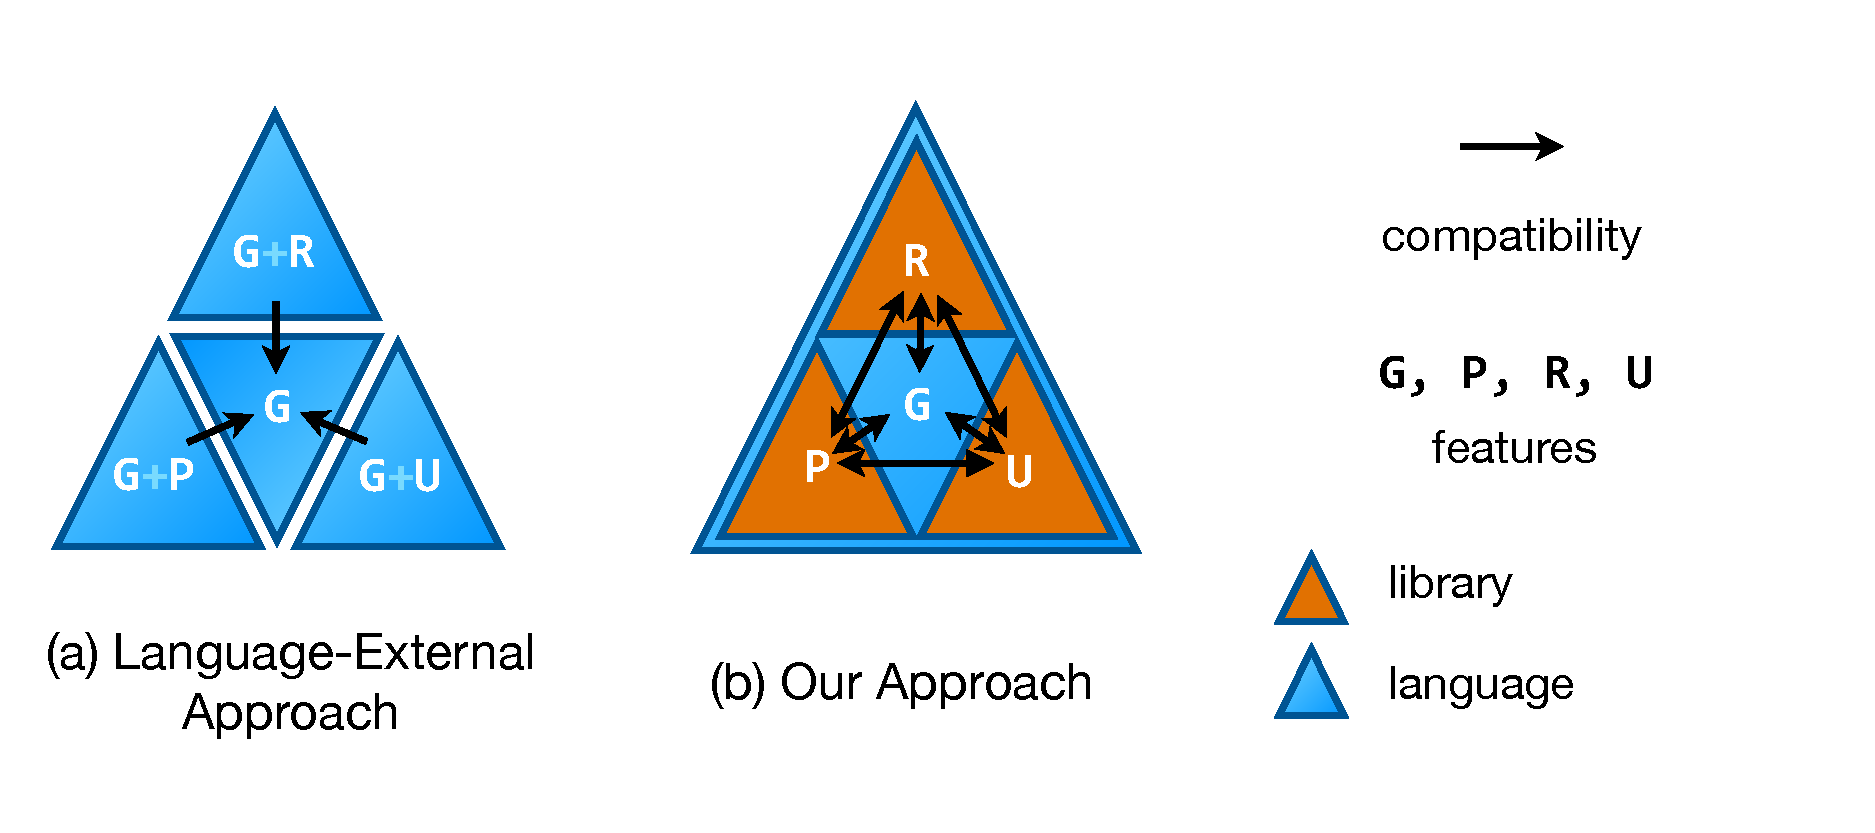
\includegraphics[scale=.48]{approaches.pdf}
% % \end{center}
% % \vspace{-20px}
% % \caption{\small (a) When taking a language-external approach, new features are packaged together into separate languages and tools. (b) We propose an approach where there is one extensible host language and the compile-time and edit-time logic governing new constructs is expressed within safely composable libraries.}
% % \label{approaches}
% % %\vspace{-10px}
% % \end{figure}
% %  %
% % % More specifically, there is no guarantee of \textbf{orthogonality} or even \textbf{interoperability}.% This has limited the broad adoption of these kinds of innovations.%This latter method couples the semantics of the feature to the implementation details of a particular tool. Because the use of one implementation entails a different semantics for the feature than another, the extended tool acts, \emph{de facto}, as a distinct system for our purposes. 

% % %\paragraph{Orthogonality} Features implemented by language-external means like these cannot be adopted individually, but instead are only available coupled to a fixed collection of other features. This makes adoption more costly when these incidental features are  not desirable or are insufficiently developed (``toy languages''), or when the features bundled with a different language or tool are simultaneously desirable. 

% % % Recent evidence indicates that this is one of the major barriers preventing research  from being driven into practice. For example, developers prefer high-level language-integrated parallel programming abstractions that provide  stronger semantic guarantees  \cite{cave2010comparing}, but library-based approximations are far more widely adopted because the ``parallel programming languages'' privilege only a few  specialized abstractions at the language level. In contrast, it is widely acknowledged that  different specialized abstractions are more appropriate in different situations \cite{Tasharofi:2013rc}. Moreover,  parallel programming is rarely the only relevant specialized concern. Support for regular expressions as above would be simultaneously desirable for processing large amounts of genomic data in parallel.% but using these features together in the same compilation unit would be difficult or impossible if implemented using language-external means. Indeed, switching to a ``parallel programming language'' would likely make it \emph{more} difficult to use regular expressions, as these are likely to be less well-developed in a specialized language than in an established general-purpose language.% This intuition was perhaps most succinctly expressed by a participant in a recent study by Basili et al. \cite{basili2008understanding}:  ``I hate MPI, I hate C++. [But] if I had to choose again, I would probably choose the same.'' %Similarly, a language and tools designed primarily to support regular expressions might make an interesting research project, but it would not be a suitable tool for writing large applications with more varied needs.

% % %\item Developing a new language and its associated tools places a significant development burden on providers who may wish only to promote a few core innovations, although tools like compiler generators, language workbenches and easy-to-extend tools can decrease this burden. 
% % %\item 

% % %Clients seem to prioritize the ability to choose different features for different portions of an application. 
% % %If calling between languages were safe and easy, then using a variety of specialized languages and associated tools might be less problematic. In fact, s
% % %Recognizing the limitations of relying on monolithic collection of primitives, some researchers have advocated instead for a model where multiple languages used within a single application, calling it the \emph{language-oriented approach} to software development \cite{languageoriented}. 

% % % \paragraph{Interoperability} Even in cases where, for each component of a software system, a programming system considered entirely satisfactory by its developers is available (e.g. a team goes through the trouble of implementing \verb|G+R+P| by reading papers about \verb|G+R| and \verb|G+P| and disentangling orthogonality-related issues), there remains a problem at any interface between  components written using a different combination of features. An interface that  externally exposes a specialized construct particular to one language (e.g. a function that requires a quantity having a particular unit of measure) cannot necessarily be safely and naturally consumed from another language (e.g. a parallel programming language). Tool support is also lost when calling into different languages. %We call this the \emph{interoperability problem}. % programs written by clients of a certain collection of features cannot always interface with programs written by clients of other features  in a safe, performant and natural manner.

% % % One strategy taken by proponents of a {language-oriented approach} \cite{journals/stp/Ward94} to partially address the interoperability problem is to  target an established intermediate language and use its constructs as a common language for communication between components written in different languages. Scala \cite{200464/IC} and F\# \cite{pickering2007foundations} are examples of prominent general-purpose languages that have taken this approach, and most DSL frameworks also rely on this strategy. As indicated in Figure \ref{approaches}a, this only enables interoperability in one direction. Calling into the common language becomes straightforward and safe, but calling in the other direction, or between the languages sharing the common target, does not, unless these languages are only trivially different from the common language. 

% % % %This approach only works well when new languages consist of constructs that can also be expressed safely and almost as naturally in the common language.
% % % %But many of the most innovative constructs found in modern languages (often, those that justify their creation) are difficult to define in terms of existing constructs in ways that guarantee all necessary invariants are statically maintained and that do not require large amounts boilerplate code and run-time overhead. 
% % % As a simple example with significant contemporary implications, F\#'s type system does not admit \verb|null| as a value for any type both defined and used within F\# code, but maintaining this sensible internal invariant still requires dynamic  checks because the stricter typing rules of F\# do not apply when F\# data structures are constructed by other languages on the Common Language Infrastructure (CLI) like C\# or SML.NET. This is not an issue exclusive to intermediate languages that make regrettable choices regarding \verb|null|, however. The F\# type system also includes support for checking that units of measure are used correctly \cite{syme2012expert, kennedy1994dimension}, but this more specialized static invariant is left entirely unchecked at language boundaries. Indeed, guidelines for F\# suggest that exposing functions that operate over values having units of measure, datatypes or tuples is not recommended when a component ``might be used'' from another language \cite{syme2012expert} because it is awkward to construct and consume these from other languages without the convenient primitive operations (e.g. pattern matching) and syntax that F\# includes. SML.NET prohibits exposing such types at component boundaries altogether. Moreover, it also cannot naturally consume F\# data structures, despite having a rather similar syntax and semantics in most ways (both languages directly descend from ML). 
% % %In Scala, traits that have default method implementations are difficult to implement from Java or other JVM languages and the workaround can break if the trait is modified \cite{scalatraitinterop}. 
% % %In some cases, desirable features must be omitted entirely due to concerns about interoperability. F\#, for example, aimed to retain source compatibility with OCaml code, but due to the need for bidirectional interoperability with CLI languages, it does not support features like polymorphic variants, modules or functors \cite{OCaml-manual} because they have no apparent analogs in the type system of the CLI.
% % %\end{itemize}

% % %\subsection{Language-Integrated Approaches}\label{language-integrated-approaches}


% % %Such libraries have been called \emph{active libraries}  \cite{activelibraries}. %Features implemented within active libraries can be imported individually, unlike features implemented by external means, giving us a potential means to avoid the problems of orthogonality and interoperability just described.

% % % We must proceed with caution, however: critical issues having to do with {safety} must be overcome before language-integrated extension mechanisms can be introduced into a system. If too much control over  these core features of the system is given  to developers, the system's metatheory may become weak. 
% % % %For example, an extension could weaken important metatheoretic guarantees previously provided by the system. 
% % % For example, parsing ambiguities might arise if the syntax can be modified arbitrarily. Type safety  may not hold if the static and dynamic semantics of the language can be modified or extended arbitrarily from within libraries. Furthermore, even if extensions can be shown not to cause such problems in isolation, there may still be conflicts between extensions that could weaken their semantics, leading to subtle problems that only appear when two extensions are used together. %As a simple example, if two active libraries introduce the same syntactic form but back it with differing (but individually valid) semantics, this ambiguity  would only manifest itself when both libraries were imported within the same scope. %Resolving these kinds of ambiguities requires significantly more expertise with parser technology than using the syntax itself does. 
% % % These issues have plagued previous attempts to design language-integrated extensibility mechanisms.\todo{I can include a more detailed related work section if requested.}% We will briefly review some of these attempts below, then return to our approach.% To prevent them, our mechanisms will organize  extension logic around types to guarantee that extensions are both safe in isolation and also safely composable in any combination. 


% %  %This represents a minimalist approach to system design -- the conventional distinction between built-in and user-defined constructs is blurred and most features of the system are orthogonally implemented as {libraries}, rather than by the maintainers of the system.

% % %The mechanisms we describe will do so primarily by delimiting the scope of an extension to expressions of a single user-defined type or family of types. 

% % %This can be thought of as a more pernicious form of the conflict that arises when two globally-accessible constructs are given the same name. n languages without universal namespacing mechanisms (e.g. C, JavaScript, \LaTeX, ML and many others). 

% % %The extension mechanism\todo{elaborate on safety requirements + tension between expressiveness and safety, merge with next paragraph}. must be expressive enough to allow users to associate rich run-time, compile-time and edit-time behaviors with user constructs directly, while being sufficiently restrictive to maintain the global safety properties of the language and system as a whole, and to ensure that constructs cannot interfere with one another. 

% \begin{figure}[p!]
% \vspace{-25px}
% \begin{lstlisting}
% metasignature LTUPLE = metasig {
%   ^\label{line:ltuplex-c-sig}^tycon c of ComponentSpec
%   ^\label{line:intro-unlabeled-sig}^ana opcon intro_unlabeled of unit
%   ^\label{line:intro-labeled-sig}^syn opcon intro_labeled of list(Lbl)
%   ^\label{line:prj-sig}^syn opcon # of Lbl
%   ^\label{line:conc-sig}^syn opcon + of unit
%   ^\label{line:drop-sig}^syn opcon - of Lbl
% }

% ^\label{line:ltplx-tsm-start}^syntax ltpl(L :: LTUPLE, param :: ComponentSpec) at L.c(param) {
%   static fn ps => (* 
%     - elaborates {e_1, ..., e_n} to 
%         L.intro_unlabeled () (e_1; ...; e_n)
%     - elaborates {lbl1 => e_1, ..., lbln => e_n} to 
%         L.intro_labeled [lbl1, ..., lbln] e_1 ... e_n
%   *)
% }^\label{ltplx-tsm-end}^

% metamodule Ltuple :: LTUPLE = metamod {
%   ^\label{line:c-start}^(* translate labeled tuple types to nested products *)
%   tycon c {
%   	(* type translation generator: *)
%   	static fn (param :: ComponentSpec) :: ITy => fold (comp_spec_to_tuples param)
%       `SCSSunitECSS`
%       (fn ((lbl, ty), cur_ty_trans) => `SCSStrans(ECSStySCSS) * %ECSScur_ty_trans`)
%   }^\label{line:c-end}^

%   ^\label{line:introul-start}^ana opcon intro_unlabeled {
%   	(* translate intro operator to nested pairs *)
%   	static fn (ty :: Ty, op_param :: unit, args :: list(Arg)) :: IExp => tycase(ty) {
%         c(ty_param) => (fold (zipExact (comp_spec_to_tuples ty_param) args)
%       	  `SCSS()ECSS`
%           (fn (((lbl, ty), arg), cur_trans) => `SCSS(%{ECSSana(arg, ty)SCSS}, %ECSScur_transSCSS)ECSS`)
%         )
%       | _ => raise TyErr("...")
%     }
%   }^\label{line:introul-end}^

%   ^\label{line:introl-start}^syn opcon intro_labeled {
%   	static fn (op_param :: list(Lbl), args :: list(Arg)) :: Ty * IExp => 
%       (* ... similar to intro_unlabeled but reorder first ... *)
%   }^\label{line:introl-end}^

%   ^\label{line:prj-start}^syn opcon # {
%   	static fn (op_param :: Lbl, args :: list(Arg)) :: Ty * IExp =>  
%       (* ... generate the appropriate n-fold projection ... *)
%   }^\label{line:prj-end}^

%   ^\label{line:ltpl-conc-start}^syn opcon + {
%   	static fn (op_param :: unit, args :: list(Arg)) :: Ty * IExp => 
%       (* generate the new type and combine the two nested tuples *)
%   }^\label{line:ltpl-conc-end}^

%   ^\label{line:ltpl-drop-start}^syn opcon - {
%   	static fn (op_param :: Lbl, args :: list(Arg)) :: Ty * IExp => 
%       (* generate the new type and drop the appropriate component *)
%   }^\label{line:ltpl-drop-end}^
% } with syntax ltpl^\label{line:ltplx-annotation}^
% (* synonyms used in Sec. 5.1 *)
% ^\label{line:tycon-synonym}^let tycon ltuple = Ltuple.c
% let opcon # = Ltuple.#
% let opcon ltuple+ = Ltuple.+ 
% let opcon ltuple- = Ltuple.-
% \end{lstlisting}
% \caption{Using metamodules to define the type structure of labeled tuple types.}
% \label{fig:ltuplex}
% \end{figure}